%
\documentclass[11pt]{article}
\newcommand{\teilnr}{I}
\usepackage{xr}
\externaldocument{../teil2/main_teil2}
\externaldocument{../teil3/main_teil3}
%
%
\usepackage[margin=1.2in]{geometry}
\usepackage{graphicx}
%
\makeatletter\newcommand*{\captionfigur}{\def\@captype{figure}\caption}\makeatother
\usepackage{tikz}\usetikzlibrary{fit,calc,arrows.meta,backgrounds}   %
%
\renewcommand{\topfraction}{0.85}\renewcommand{\textfraction}{0.1}\renewcommand{\floatpagefraction}{0.75}
\graphicspath{{../abbildungen/}}   %
\usepackage[T1]{fontenc}
\usepackage{lmodern}
\usepackage{amsmath,amssymb,amsthm}
\usepackage{etoolbox}
\usepackage{refcount}
\usepackage{array}       %
\usepackage{longtable}   %
\usepackage[hidelinks]{hyperref}

\providecommand{\teilnr}{?}
\newif\ifimband

%
\newtheorem{theorem}{Theorem}[section]
\newtheorem{proposition}[theorem]{Proposition}
\newtheorem{lemma}[theorem]{Lemma}
\newtheorem{corollary}[theorem]{Corollary}
\theoremstyle{definition}
\newtheorem{definition}[theorem]{Definition}
\theoremstyle{remark}
\newtheorem{remark}[theorem]{Remark}
\newtheorem{question}[theorem]{Question}
\renewcommand{\thetheorem}{\teilnr.\arabic{section}.\arabic{theorem}}
\numberwithin{equation}{section}
%
%
\def\theHtheorem{\teilnr.\arabic{section}.\arabic{theorem}}
\def\theHsection{\teilnr.\arabic{section}}
\def\theHequation{\teilnr.\arabic{section}.\arabic{equation}}

%
%
%
%
\newcommand{\tlabel}[1]{\label{\teilnr:#1}}
%
%
%
\newwrite\belegaus
\immediate\openout\belegaus=\jobname.bel
\newcommand{\belegart}[1]{\immediate\write\belegaus{\thetheorem|#1|\thesection}{\normalfont\small[#1]}\ }
\newcommand{\tref}[1]{\ref{\teilnr:#1}}
\makeatletter
\newcommand{\partref}[2]{%
  \edef\serie@teil{\teilnr}\def\serie@ziel{#1}%
  \ifx\serie@teil\serie@ziel\ref{#1:#2}%
  \else\ifimband\ref{#1:#2}%
  \else\getrefnumber{#1:#2}~in~[Part~#1]\fi\fi}
\makeatother

%
%
%
%
\makeatletter
%
\@namedef{Z@nenner}{811}
%
\@namedef{Z@offen}{6}
%
\@namedef{Z@erledigt}{805}
%
\@namedef{Z@zertifiziert}{767}
%
\@namedef{Z@vollzerlegt}{38}
%
\@namedef{Z@csechsquadrat}{1.3685}
%
\@namedef{Z@csechswalker}{0.3137}
%
\@namedef{Z@csechs}{1.6822}
%
\@namedef{Z@streifenfam}{206}
%
\@namedef{Z@streifentot}{52}
%
\@namedef{Z@streifentuerme}{154}
%
\@namedef{Z@streifenstellen}{8.4\cdot 10^{7}}
%
\@namedef{Z@streifenminm}{223}
%
\@namedef{Z@streifensieben}{17.5}
%
\@namedef{Z@streifeneins}{2}
%
\@namedef{Z@margestich}{530}
%
\@namedef{Z@margemax}{10^{8}}
%
\@namedef{Z@margerand}{2\cdot 10^{5}}
%
\@namedef{Z@margemin}{21.5}
%
\@namedef{Z@streifenschranke}{2000}
%
\@namedef{Z@streifensteckt}{14}
%
\@namedef{Z@glattkerne}{889\,437}
%
\@namedef{Z@glattkand}{0}
%
\@namedef{Z@glattunten}{10^{8}}
%
\@namedef{Z@glattoben}{10^{15}}
%
\@namedef{Z@glatthoehe}{2000}
%
\@namedef{Z@glattprim}{100}
%
\@namedef{Z@glattmin}{4}
%
\@namedef{Z@glattperiode}{9573}
%
\@namedef{Z@glattgross}{356\,888}
%
\@namedef{Z@glattrest}{532\,549}
%
\@namedef{Z@bboxkern}{10^{6}}
%
\@namedef{Z@bboxb}{10^{4}}
%
\@namedef{Z@bboxfam}{101\,329}
%
\@namedef{Z@bboxparitaet}{32\,118}
%
\@namedef{Z@bboxpaare}{421\,010\,513}
%
\@namedef{Z@bboxohnealpha}{343\,504\,538}
%
\@namedef{Z@bboxzweiadisch}{16\,603\,302}
%
\@namedef{Z@bboxkgerade}{11\,242\,224}
%
\@namedef{Z@bboxlemmal}{49\,659\,524}
%
\@namedef{Z@bboxrest}{925}
%
\@namedef{Z@ballotfaelle}{56}
%
\@namedef{Z@ballotgedruckt}{0}
%
\@namedef{Z@ballotfib}{50}
%
\@namedef{Z@turmk1}{1.1\cdot 10^{13}}
%
\@namedef{Z@turmk2}{5.5\cdot 10^{13}}
%
\@namedef{Z@turmk3}{4.5\cdot 10^{30}}
%
\@namedef{Z@turmstellen}{2.5\cdot 10^{15}}
%
\@namedef{Z@kongruenzbis}{10^{5}}
%
\@namedef{Z@kongruenzdichte}{2.67\cdot 10^{-4}}
%
\@namedef{Z@yokoimax}{20000}
%
\@namedef{Z@yokoipaare}{123}
%
\@namedef{Z@designkerne}{251}
%
\@namedef{Z@designtmax}{399}
%
\@namedef{Z@designfenster}{17}
%
\@namedef{Z@designmaxm}{1023}
%
\@namedef{Z@designstellen}{2000}
%
\@namedef{Z@quadratzeuge1}{701}
%
\@namedef{Z@quadratzeuge2}{3}
%
\@namedef{Z@quadratzeuge3}{5}
%
\@namedef{Z@mittenquadrat}{0.3648}
%
\@namedef{Z@mittendoppel}{0.2580}
%
\@namedef{Z@mittensatza}{0.6228}
%
\@namedef{Z@mittenN}{10^{14}}
%
\@namedef{Z@mittengemessen}{0.6252}
%
\@namedef{Z@kerne}{10\,132\,126}
%
\@namedef{Z@kernschranke}{10^{8}}
%
\@namedef{Z@hoehe}{2000}
%
\@namedef{Z@zeugenschranke}{2\cdot 10^{5}}
%
\@namedef{Z@filterfamilien}{83}
%
\@namedef{Z@punktfamilien}{79}
%
\@namedef{Z@punkte}{445}
%
\@namedef{Z@paritaetspunkte}{74}
%
\@namedef{Z@zeugenpunkte}{371}
%
\@namedef{Z@restpunkte}{0}
%
\@namedef{Z@beispielm}{7}
%
\@namedef{Z@beispielk}{7}
%
\@namedef{Z@beispielzeuge}{29}
%
\@namedef{Z@beispielwert}{130\,576\,328}
%
\@namedef{Z@beispielfaktoren}{2^{3}\cdot 29\cdot 197\cdot 2857}
%
\@namedef{Z@ohnetripel}{3.88\cdot 10^{20}}
%
\@namedef{Z@ohnetripelsicher}{1.83\cdot 10^{18}}
%
\@namedef{Z@famtab}{(2, 1) & 1 & 0.90 & 1.53 & 14 \\
(3, 1) & 3 & 2.83 & 3.43 & 6 \\
(23, 2) & 1 & 4.09 & 9.37 & 2 \\
(6, 1) & 3 & 5.37 & 5.97 & 3 \\
(1, 5) & 5 & 5.67 & 12.54 & 2 \\
(46, 1) & 1 & 8.77 & 9.37 & 2 \\
(7, 2) & 7 & 9.73 & 20.67 & 1 \\
(5, 1) & 5 & 11.94 & 12.54 & 1 \\
(430, 1) & 1 & 12.91 & 13.52 & 1 \\
(79, 23) & 1 & 13.08 & 27.36 & 1 \\
(3, 7) & 7 & 13.69 & 28.58 & 1 \\
(10, 1) & 5 & 15.19 & 15.79 & 1 \\
(7, 1) & 7 & 16.23 & 16.83 & 1 \\
(14, 1) & 7 & 20.07 & 20.67 & 1 \\
(1022, 57) & 1 & 20.21 & 41.62 & 1 \\
(19, 35) & 5 & 21.59 & 44.38 & 1 \\}
%
\@namedef{Z@famzahl}{16}
%
\@namedef{Z@famtabzwei}{14}
%
\@namedef{Z@fampaare}{39}
%
\@namedef{Z@famquadrat}{32}
%
\@namedef{Z@famohne}{7}
%
\@namedef{Z@paargrenze}{3.89\cdot 10^{21}}
%
\@namedef{Z@paarletzt}{3\,887\,785\,221\,910\,670\,811\,499}
%
\@namedef{Z@periodepk}{6082}
%
\@namedef{Z@periodepkmax}{10\,000}
%
\@namedef{Z@walkerpk}{955}
%
\@namedef{Z@walkerpkmax}{3000}
%
\@namedef{Z@paare52}{26}
%
\@namedef{Z@paare52exp}{52}
%
\@namedef{Z@mersennemax}{63}
%
\@namedef{Z@famquadratfam}{10}
%
\@namedef{Z@quadratbmax}{10^{4}}
%
\@namedef{Z@walkerdmax}{10^{6}}
%
\@namedef{Z@expfam}{750}
%
\@namedef{Z@expmmax}{10^{4}}
%
\@namedef{Z@exppmax}{3000}
%
\@namedef{Z@exppaare}{120\,373}
%
\@namedef{Z@expwzwei}{470}
%
\@namedef{Z@expwdrei}{52}
%
\@namedef{Z@exphzwei}{486}
%
\@namedef{Z@exphdrei}{49.1}
%
\@namedef{Z@korrs}{411.7}
%
\@namedef{Z@korrmu}{436.2}
%
\@namedef{Z@korrsd}{28.2}
%
\@namedef{Z@korrreps}{4000}
%
\@namedef{Z@korrz}{-0.87}
%
\@namedef{Z@korrp}{0.80}
%
\@namedef{Z@korrvert}{396, 255, 83, 15, 1}
%
\@namedef{Z@korrmaxp}{181}
%
\@namedef{Z@korrmaxz}{2.4}
%
\@namedef{Z@trennvoll}{652}
%
\@namedef{Z@trennzwei}{90}
%
\@namedef{Z@trennfuenf}{48}
%
\@namedef{Z@trennlaeufe}{40}
%
\@namedef{Z@alekterme}{33}
%
\@namedef{Z@alekstellen}{67}
%
\@namedef{Z@klassedreimax}{10^{8}}
%
\@namedef{Z@alekneun}{9}
%
\@namedef{Z@vollexpo}{36}
%
\@namedef{Z@vollmexpo}{24}
%
\@namedef{Z@reinhartt1}{94}
%
\@namedef{Z@reinharttab}{4\,099\,215 & 228 & $2\cdot 10^{5}$ & 701, 100469, 157049 & $1.1\cdot 10^{13}$ & $2.5\cdot 10^{15}$ \\
39\,028\,039\,587\,479 & 1\,880\,030 & $3\cdot 10^{3}$ & 5, 7, 71, 1657; 19, 29, 421, 569, 1987; 379, 2089, 2203, 2437 & $4.5\cdot 10^{30}$ & $8.6\cdot 10^{36}$ \\}
%
\@namedef{Z@reinhartungerade}{209\,991}
%
\@namedef{Z@reinhartungerade2}{117\,477\,414\,815}
%
\@namedef{Z@reinhartboxk}{1, 3, 5, 7}
%
\@namedef{Z@reinhartboxz}{701, 11, 19, 29}
%
\@namedef{Z@reinhartungeradest}{95}
%
\@namedef{Z@reinhartungeradest2}{11\,621}
%
\@namedef{Z@zeugenalle}{371}
%
\@namedef{Z@zeugenprim}{8}
%
\@namedef{Z@zeugenmedian}{19}
%
\@namedef{Z@zeugenmax}{114\,997}
%
\@namedef{Z@zeugen29}{79}
%
\@namedef{Z@zeugen19}{78}
%
\@namedef{Z@zeugen11}{45}
%
\@namedef{Z@zeugen3}{43}
%
\@namedef{Z@zeugen5}{33}
%
\@namedef{Z@zeugen7}{25}
%
\@namedef{Z@zeugennkp}{197}
%
\@namedef{Z@zeugennkk}{1379}
%
\@namedef{Z@zeugennkv}{2}
%
\@namedef{Z@rizzierfuellt}{328}
%
\@namedef{Z@rizzinicht}{43}
%
\@namedef{Z@kongrp}{10^{6}}
%
\@namedef{Z@kongrkerne}{15}
%
\@namedef{Z@kongrpaare}{425\,362}
%
\@namedef{Z@bedpunkte}{445}
%
\@namedef{Z@bedteiler}{2149}
%
\@namedef{Z@bedausweg}{1682}
%
\@namedef{Z@bedanteil}{78.3}
%
\@namedef{Z@bedmedian}{3}
%
\@namedef{Z@bedmittel}{3.8}
%
\@namedef{Z@bedmax}{12}
%
\@namedef{Z@bedallemedian}{4}
%
\@namedef{Z@bedallemax}{16}
%
\@namedef{Z@besp}{3\cdot 10^{6}}
%
\@namedef{Z@beskerne}{25}
%
\@namedef{Z@besnp}{5}
%
\@namedef{Z@bespunkte}{378}
%
\@namedef{Z@besraenge}{2536}
%
\@namedef{Z@besbesetzt}{2025}
%
\@namedef{Z@beszeuge}{1988}
%
\@namedef{Z@beszeugeant}{98.17}
%
\@namedef{Z@beswief}{37}
%
\@namedef{Z@besleer}{511}
%
\@namedef{Z@beseinsnp}{1}
%
\@namedef{Z@beseinszeuge}{1936}
%
\@namedef{Z@beseinsant}{95.60}
%
\@namedef{Z@beseinswief}{89}
%
\@namedef{Z@rgpaare}{961}
%
\@namedef{Z@rgkerne}{79}
%
\@namedef{Z@rgerledigt}{954}
%
\@namedef{Z@rgzert}{954}
%
\@namedef{Z@rgvoll}{0}
%
\@namedef{Z@pbbausteine}{41}
%
\@namedef{Z@pbzahlen}{24}
%
\@namedef{Z@pbpock}{18}
%
\@namedef{Z@pbecpp}{6}
%
\@namedef{Z@pbpockmax}{75}
%
\@namedef{Z@pbecppmax}{477}
%
\@namedef{Z@rgoffen}{7}
%
\@namedef{Z@rgprpzeuge}{0}
%
\@namedef{Z@rgbedingt}{0}
%
\@namedef{Z@teilevollm}{23}
%
\@namedef{Z@teilevolld}{161}
%
\@namedef{Z@teilevolla}{111}
%
\@namedef{Z@teilevollb}{112}
%
\@namedef{Z@teilezeugem}{7}
%
\@namedef{Z@teilezeuged}{1449}
%
\@namedef{Z@teilezeugest}{477}
%
\@namedef{Z@rgaltkerne}{25}
%
\@namedef{Z@rgneukerne}{54}
%
\@namedef{Z@rgungerade}{21}
%
\@namedef{Z@wegetab}{certified witness: search by position, small primes & 605 & 103 & 708 \\
certified witness: search by position, congruence filter & 64 & 16 & 80 \\
certified witness: elliptic curves and $p - 1$ (SymPy) & 70 & 0 & 70 \\
certified witness: elliptic curves (GMP-ECM) & 27 & 20 & 47 \\
certified witness: $M_d$ itself prime, with a certificate & 8 & 8 & 16 \\
certified witness: complete factorization, factors proved prime & 32 & 0 & 32 \\
certified witness: a factor of the algebraic split, proved prime & 1 & 0 & 1 \\
open & 4 & 3 & 7 \\}
%
\@namedef{Z@bouchardn}{9800}
%
\@namedef{Z@bouchardp}{13}
%
\@namedef{Z@bouchardfakt}{2\cdot 13^{2}\cdot 29}
%
\@namedef{Z@pellwief}{13,\ 31,\ 1546463}
%
\@namedef{Z@reinhartza}{701}
%
\@namedef{Z@reinhartzc}{5}
%
\@namedef{Z@offentab}{399 & 171 & 173 & 300 & 1071 & 2753 & 8.36 & 1.10 \\
407 & 111 & 269 & 300 & 1071 & 2753 & 8.36 & 1.10 \\
39 & 247 & 367 & 300 & 1071 & 2753 & 8.36 & 1.10 \\
111 & 185 & 400 & 300 & 1071 & 2753 & 8.36 & 1.10 \\
407 & 259 & 805 & 300 & 1071 & 2753 & 8.05 & 1.05 \\
663 & 663 & 889 & 300 & 1071 & 38 & 1.05 & 0.11 \\
20\,303 & 257 & 1893 & 300 & 209 & -- & 0.22 & 0.02 \\}
%
\@namedef{Z@wfinpop}{3}
%
\@namedef{Z@offenmin}{173}
%
\@namedef{Z@erstesucheP}{3\cdot 10^{6}}
%
\@namedef{Z@siebober}{10^{9}}
%
\@namedef{Z@prtripel}{1341}
%
\@namedef{Z@prvauf1}{1338}
%
\@namedef{Z@prvauf2}{3}
%
\@namedef{Z@prerwartet}{2.38}
%
\@namedef{Z@zweip}{10^{6}}
%
\@namedef{Z@zweiamax}{100\,000}
%
\@namedef{Z@zweiexp}{99\,999}
%
\@namedef{Z@zweiminus}{8957}
%
\@namedef{Z@zweiminusant}{8.96}
%
\@namedef{Z@zweiplus}{2511}
%
\@namedef{Z@zweiplusant}{2.51}
%
\@namedef{Z@zweiminusok}{91\,042}
%
\@namedef{Z@zweiplusok}{97\,488}
%
\@namedef{Z@zweistellen}{30\,103}
%
\@namedef{Z@wfereignisse}{54}
%
\@namedef{Z@wfprimzahlen}{40}
%
\@namedef{Z@wfkerne}{79}
%
\@namedef{Z@wfp}{3\cdot 10^{6}}
%
\@namedef{Z@wfungerade}{18}
%
\@namedef{Z@wfgerade}{15}
%
\@namedef{Z@wfzeuge}{11}
%
\@namedef{Z@wfoffen}{3}
%
\@namedef{Z@wfentschieden}{12}
%
\@namedef{Z@wfmgross}{1\,375\,502\,561}
%
\@namedef{Z@wfmgroesser}{158\,585\,313\,121}
%
\@namedef{Z@wfmquadrat}{20161}
%
\@namedef{Z@erstesuchekerne}{25}
%
\@namedef{Z@lucasgleich}{16}
%
\@namedef{Z@lucaspk}{3}
%
\@namedef{Z@lucasnk}{25}
%
\@namedef{Z@wftab}{15 & 45 & 181 & witness & yes \\
31 & 39 & 157 & witness & no \\
79 & 253 & 4049 & witness & no \\
143 & 13 & 311 & witness & yes \\
223 & 45 & 179 & witness & no \\
319 & 5 & 20\,161 & complete factorization & yes \\
383 & 21545 & 258\,539 & witness & no \\
447 & 413 & 24\,781 & witness & no \\
455 & 9 & 37 & witness & no \\
615 & 807 & 3229 & not settled & no \\
1343 & 5 & 19 & witness & no \\
1535 & 63 & 251 & witness & no \\
2135 & 13 & 53 & witness & no \\
2135 & 37 & 149 & not settled & no \\
123\,879 & 9 & 37 & not settled & no \\}
%
\@namedef{Z@wfinpopzu}{3}
%
\@namedef{Z@wfnullrang}{16}
%
\@namedef{Z@csechsbmax}{10^{6}}
%
\@namedef{Z@csechsfamq}{676\,094}
%
\@namedef{Z@csechsfamw}{275\,371}
%
\@namedef{Z@kdkerne}{10\,132\,121}
%
\@namedef{Z@kdschranke}{10^{8}}
%
\@namedef{Z@kdkandidaten}{86}
%
\@namedef{Z@kdpunkte}{883}
%
\@namedef{Z@kdungerade}{51}
%
\@namedef{Z@kdpaare}{832}
%
\@namedef{Z@kdkernmax}{3\,926\,299}
%
\@namedef{Z@kdpaarkerne}{57}
%
\@namedef{Z@kddrei}{583}
%
\@namedef{Z@kdreinhartst}{99\,134}
%
\@namedef{Z@kdreinhartungst}{117}
%
\@namedef{Z@turmtab}{100 & 14 & 37 & 21 & 67 \\
250 & 39 & 97 & 53 & 168 \\
500 & 83 & 199 & 111 & 344 \\
1000 & 176 & 410 & 224 & 695 \\
1500 & 270 & 616 & 345 & 1049 \\
2000 & 371 & 832 & 467 & 1404 \\}
%
\@namedef{Z@turmc7}{0.1817}
%
\@namedef{Z@turmc3}{0.4134}
%
\@namedef{Z@turmc}{0.595}
%
\@namedef{Z@turmtuerme}{122}
%
\@namedef{Z@turmtuerme7}{60}
%
\@namedef{Z@turmtuerme3}{62}
%
\@namedef{Z@turmueber}{111.8}
%
\@namedef{Z@wtab}{1 & 0.0594 & 0.2914 \\
2 & 0.1341 & 0.3666 \\
3 & 0.1711 & 0.4027 \\
4 & 0.1936 & 0.4212 \\
5 & 0.2047 & 0.4366 \\
6 & 0.2151 & 0.4513 \\
7 & 0.2217 & 0.4566 \\}
%
\@namedef{Z@modellp}{31}
%
\@namedef{Z@modell7min}{0.94}
%
\@namedef{Z@modell7max}{1.01}
%
\@namedef{Z@modell3min}{0.91}
%
\@namedef{Z@modell3max}{1.04}
%
\@namedef{Z@beins7}{87.1}
%
\@namedef{Z@beins3}{86.3}
%
\@namedef{Z@einkernm}{525\,003}
%
\@namedef{Z@einkernanteil}{45}
%
\@namedef{Z@modellc}{0.7482}
%
\@namedef{Z@modellrate}{0.8835}
%
\@namedef{Z@naivrate}{1.1808}
%
\@namedef{Z@modelltab}{8 & 10 & 11.5 & 15.4 \\
10 & 14 & 15.5 & 20.7 \\
12 & 18 & 19.5 & 26.0 \\
14 & 24 & 23.5 & 31.4 \\
16 & 26 & 27.6 & 36.9 \\
18 & 31 & 31.6 & 42.3 \\
20 & 35 & 35.7 & 47.7 \\}
%
\@namedef{Z@modellnull}{39}
%
\@namedef{Z@modellnullkorr}{38.94}
%
\@namedef{Z@modellnullnaiv}{52.04}
%
\@namedef{Z@modellneu}{13}
%
\@namedef{Z@modellneukorr}{12.06}
%
\@namedef{Z@modellneunaiv}{16.12}
%
\@namedef{Z@quadbmax}{10^{4}}
%
\@namedef{Z@quadtab}{49.7 & 32 & 38.9 & 52.0 & 0.7049 \\
75.0 & 54 & 61.3 & 81.9 & 0.7744 \\
100.0 & 76 & 83.4 & 111.4 & 0.8136 \\
150.0 & 124 & 127.5 & 170.4 & 0.8755 \\
200.0 & 171 & 171.7 & 229.5 & 0.9011 \\
300.0 & 265 & 260.1 & 347.6 & 0.9300 \\
500.0 & 468 & 436.8 & 583.7 & 0.9765 \\
1000.0 & 997 & 878.5 & 1174.1 & 1.0345 \\}
%
\@namedef{Z@quadkreuz}{192.9}
%
\@namedef{Z@quadkreuzlog}{83.8}
%
\@namedef{Z@quadgeboren}{103}
%
\@namedef{Z@quadrate1000}{1.0345}
%
\@namedef{Z@quadnq1000}{997}
%
\@namedef{Z@quadv1000}{878.5}
%
\@namedef{Z@quadrest1000}{894}
%
\@namedef{Z@teilsumq1}{0.6055}
%
\@namedef{Z@teilsumq2}{0.8949}
%
\@namedef{Z@teilsumtab}{3 & 1.1044 & 0.1783 & 1.2827 \\
4 & 1.2235 & 0.2385 & 1.4619 \\
5 & 1.3110 & 0.2831 & 1.5941 \\
6 & 1.3685 & 0.3137 & 1.6822 \\}
%
\@namedef{Z@zuwq}{79}
%
\@namedef{Z@zuww}{77}
%
\@namedef{Z@zuwtopq}{71}
%
\@namedef{Z@zuwtopw}{72}
%
\@namedef{Z@a1nmax}{10^{12}}
%
\@namedef{Z@a1dmax25}{10^{5}}
%
\@namedef{Z@a1paare25}{18}
%
\@namedef{Z@a1dmax}{20\,000}
%
\@namedef{Z@a1kerne}{12\,159}
%
\@namedef{Z@a1paare}{6063}
%
\@namedef{Z@a1hoehe}{2000}
%
\@namedef{Z@a1ueber}{7}
%
\@namedef{Z@a1paareh}{6056}
%
\@namedef{Z@a1p1}{5\cdot 10^{5}}
%
\@namedef{Z@a1zeuge1}{4991}
%
\@namedef{Z@a1p2}{5\cdot 10^{6}}
%
\@namedef{Z@a1zeuge2}{154}
%
\@namedef{Z@a1rest2}{918}
%
\@namedef{Z@a1s2prim}{24}
%
\@namedef{Z@a1s2primzert}{5}
%
\@namedef{Z@a1s2ecm}{15}
%
\@namedef{Z@a1s2offen}{879}
%
\@namedef{Z@a1s2kleinst}{81}
%
\@namedef{Z@a1s2probable}{19}
%
\@namedef{Z@a1s2ecpp}{19}
%
\@namedef{Z@a1s2ecppmax}{1687}
%
\@namedef{Z@a1s2nk}{5}
%
\@namedef{Z@quadzeilen}{8}
%
\@namedef{Z@quadab}{300}
%
\@namedef{Z@quadablog}{130}
%
\@namedef{Z@quadslack}{6}
%
\@namedef{Z@wtabmax}{10^{7}}
%
\@namedef{Z@reinhartgerade}{3}
%
\@namedef{Z@reinhartgeradesicher}{1}
%
\@namedef{Z@reinhartsieben}{4}
%
\@namedef{Z@znab}{300}
%
\@namedef{Z@znaq}{183}
%
\@namedef{Z@znaqg}{182}
%
\@namedef{Z@znamit}{34}
%
\@namedef{Z@phidreilavij}{13}
%
\@namedef{Z@phidreibrute}{10^{6}}
%
\@namedef{Z@phidreistellen}{19, 35 and 52}
%
\@namedef{Z@phidreiperiode}{7}
%
\@namedef{Z@zyktab}{3 & 18 & 343 & $7^{3}$ \\
3 & 88\,916 & 7\,906\,143\,973 & $7^{2}\cdot 13^{3}\cdot 271^{2}$ \\
4 & 682 & 465\,125 & $5^{3}\cdot 61^{2}$ \\
5 & 3 & 121 & $11^{2}$ \\
6 & 19 & 343 & $7^{3}$ \\
6 & 88\,917 & 7\,906\,143\,973 & $7^{2}\cdot 13^{3}\cdot 271^{2}$ \\}
%
\@namedef{Z@zykn}{3\,004\,199}
%
\@namedef{Z@zyktreffer}{6}
%
\@namedef{Z@zykschranke}{10^{12}}
%
\@namedef{Z@zykklasse}{10^{14}}
%
\@namedef{Z@lstab}{$10^{12}$ & 2\,158\,391 & 832\,161 & 0.31 & 900 & 69 & 1656 & 183 of 215 \\
$10^{13}$ & 6\,840\,384 & 2\,593\,517 & 0.18 & 44\,100 & 57 & 63\,900 & 189 of 211 \\
$10^{14}$ & 21\,663\,503 & 8\,235\,300 & 0.10 & 44\,100 & 48 & 63\,900 & 191 of 201 \\}
%
\@namedef{Z@lsnpw}{21\,663\,503}
%
\@namedef{Z@lswerte}{8\,235\,300}
%
\@namedef{Z@lsanteil}{0.10}
%
\@namedef{Z@lsbis}{48}
%
\@namedef{Z@lsocc}{112}
%
\@namedef{Z@lserster}{63\,900}
%
\@namedef{Z@lsg100}{103}
%
\@namedef{Z@lsg100pw}{102}
%
\@namedef{Z@lsg200}{201}
%
\@namedef{Z@lsg200pw}{191}
%
\@namedef{Z@lserwartet}{0.05}
%
\@namedef{Z@lsdecke}{63\,900 & 900 & 9 & 112 & 50.9 \\
82\,908 & 1764 & 36--41 & 98 & 49.0 \\
17\,100 & 900 & 9 & 97 & 43.3 \\
23\,324 & 1372 & 170--175 & 96 & 20.8 \\
151\,900 & 4900 & 10--11 & 90 & 45.6 \\
171\,900 & 900 & 9 & 90 & 52.2 \\
7100 & 100 & 357--381 & 89 & 61.8 \\
26\,100 & 900 & 9 & 89 & 37.1 \\
127\,800 & 1800 & 29--31 & 89 & 53.9 \\
215\,100 & 900 & 9 & 89 & 51.7 \\}
%
\@namedef{Z@lsdeckeanz}{10}
%
\@namedef{Z@lsg20}{21}
%
\@namedef{Z@lsanteilpw}{24.2--44.9}
%
\@namedef{Z@lsanteilnpw}{20.8--61.8}
%
\@namedef{Z@nvlmax}{50}
%
\@namedef{Z@nvrel}{1.2}
%
\@namedef{Z@nvsteig}{0.63}
%
\@namedef{Z@lstop1}{44\,100}
%
\@namedef{Z@zmn}{62\,118}
%
\@namedef{Z@zmmin}{20}
%
\@namedef{Z@lsbasiswerte}{62\,118}
%
\@namedef{Z@lsbasismind}{20}
%
\@namedef{Z@lsbasisanteil}{4.81}
%
\@namedef{Z@lsbasiserw}{2.4}
%
\@namedef{Z@fpn}{3531}
%
\@namedef{Z@fpmax}{3\cdot 10^{-16}}
%
\@namedef{Z@zmr2}{0.545}
%
\@namedef{Z@zmr2sd}{0.025}
%
\@namedef{Z@zmroh}{0.306}
%
\@namedef{Z@zmrohsd}{0.005}
%
\@namedef{Z@zmr2log}{0.514}
%
\@namedef{Z@zmr2logsd}{0.016}
%
\@namedef{Z@zmallesep}{0.319}
%
\@namedef{Z@zmallesepsd}{0.012}
%
\@namedef{Z@zmalleroh}{0.307}
%
\@namedef{Z@zmallerohsd}{0.004}
%
\@namedef{Z@zmdeutstufen}{3061}
%
\@namedef{Z@zmdeutkmin}{4}
%
\@namedef{Z@zmkern}{0.012}
%
\@namedef{Z@zmkof}{0.272}
%
\@namedef{Z@zmww}{0.001}
%
\@namedef{Z@zmkerne}{2986}
%
\@namedef{Z@zmkof_n}{9752}
%
\@namedef{Z@zmdecke}{0.864}
%
\@namedef{Z@zmdeutung}{0.425}
%
\@namedef{Z@zmdeutdecke}{0.898}
%
\@namedef{Z@pmstich}{401\,176}
%
\@namedef{Z@pmschritt}{54}
%
\@namedef{Z@pmanteil}{47.69}
%
\@namedef{Z@pmgcd}{4,\ 9,\ 8,\ 16,\ 25,\ 36,\ 27,\ 32}
%
\@namedef{Z@ukerne}{25}
%
\@namedef{Z@up}{2\cdot 10^{6}}
%
\@namedef{Z@upaare}{294\,920}
%
\@namedef{Z@u11}{0}
%
\@namedef{Z@u10}{38}
%
\@namedef{Z@u01}{8}
%
\@namedef{Z@uerw}{0.001}
%
\@namedef{Z@usim}{400}
%
\@namedef{Z@utrenn}{98}
%
\@namedef{Z@utrennnull}{1}
%
\@namedef{Z@ukopie}{3.8}
%
\@namedef{Z@wf3kerne}{25}
%
\@namedef{Z@wf3p}{3\cdot 10^{6}}
%
\@namedef{Z@wfn}{5\,420\,294}
%
\@namedef{Z@wftreffer}{56}
%
\@namedef{Z@wferw}{50.71}
%
\@namedef{Z@wft4b}{593}
%
\@namedef{Z@wft4e}{583.9}
%
\@namedef{Z@wfzmax}{1.37}
%
\@namedef{Z@wfklpmin}{0.014}
%
\@namedef{Z@wfklbon}{0.08}
%
\@namedef{Z@wfklanz}{6}
%
\@namedef{Z@wglags}{20}
%
\@namedef{Z@wgtests}{500}
%
\@namedef{Z@wgueber}{7}
%
\@namedef{Z@wgerw}{5}
%
\@namedef{Z@wgzmax}{3.30}
%
\@namedef{Z@wgpbon}{0.48}
%
\@namedef{Z@wgpk}{21.4}
%
\@namedef{Z@wkpaare}{300}
%
\@namedef{Z@wkzmax}{3.61}
%
\@namedef{Z@wkpbon}{0.09}
%
\@namedef{Z@wkpk}{10.0}
%
\@namedef{Z@achtq}{2384}
%
\@namedef{Z@achtgrenze}{10^{5}}
%
\@namedef{Z@zpn}{163}
%
\@namedef{Z@zpprim}{18}
%
\@namedef{Z@zpdmax}{59}
%
\@namedef{Z@zpab16}{5}
%
\@namedef{Z@offenschwach}{0}
%
\@namedef{Z@offenneum}{399, 663 and 20\,303}
%
\@namedef{Z@zquadkerne}{26}
%
\@namedef{Z@zquadbl}{361}
%
\@namedef{Z@zquadprim}{171}
%
\@namedef{Z@zquadgrenze}{5000}
%
\@namedef{Z@reinhartsiebensicher}{3}
%
%
%
%
%
%
%
%
%
%
%
%
%
%
\makeatother

\newcommand{\Z}[1]{%
  \ifcsname Z@#1\endcsname\csname Z@#1\endcsname
  \else\PackageError{serie}{Zahl '#1' ist nicht in zahlen.tex definiert}{werkzeug/zahlen_bauen.py laufen lassen oder den Schluessel pruefen}\fi}

%
%
%
%
%
\newcommand{\inwords}{\par\medskip\noindent\textit{In words.}\ }
%
\newcommand{\spaeter}[1]{\par\noindent\textit{[#1]}\par}
\newcommand{\PrimSymbol}{M}
\newcommand{\Prim}[1]{\PrimSymbol_{#1}}
\newcommand{\Kreis}[1]{\Phi_{#1}}

%
\providecommand{\problemeletzter}{I}\providecommand{\problemeanzahl}{9}
\providecommand{\problemvon}[1]{\ifcsname prob@#1\endcsname\csname prob@#1\endcsname\else\textbf{??}\fi}
\expandafter\def\csname prob@I:q:walsh\endcsname{A}
\expandafter\def\csname prob@I:q:primindex\endcsname{B}
\expandafter\def\csname prob@I:q:zweierpotenz\endcsname{C}
\expandafter\def\csname prob@I:q:reinhart\endcsname{D}
\expandafter\def\csname prob@II:q:konvergenz\endcsname{E}
\expandafter\def\csname prob@II:q:wachstum\endcsname{F}
\expandafter\def\csname prob@II:q:ezwei\endcsname{G}
\expandafter\def\csname prob@III:q:luecken\endcsname{H}
\expandafter\def\csname prob@III:q:phiacht\endcsname{I}

\title{Triples of Consecutive Powerful Numbers: Pell Addresses, a Height Inequality, and Witnesses}
\author{Berkay Y\"uksel Sayim\\
Independent Researcher, Germany\\
\texttt{berksa@tutamail.com} $\cdot$ ORCID 0009-0004-4993-7352}
\date{October 4, 2026}
\hypersetup{pdfauthor={Berkay Y\"uksel Sayim}, pdftitle={Triples of Consecutive Powerful Numbers: Pell Addresses, a Height Inequality, and Witnesses}}
\begin{document}
\maketitle
\begin{abstract}
We study the question of Erd\H{o}s whether three consecutive integers can all be powerful. The middle $n$ of such a triple is a Pell
number $T_k(m)$ at a lattice point $(m, k)$ with a squarefree kernel $m \equiv 7 \pmod 8$. We prove a height inequality,
$\log_{10} T_k(m) \ge m'(1.5 \log_{10} m - \log_{10} m') - \log_{10} 2$, which splits the kernels into two wings by whether $m$ divides
$U_1(m)$, and we recast the reduction of Mollin and Walsh as a statement about witnesses, primes that divide a Pell number exactly once,
organized by rank. We compute: all \Z{punkte} lattice points with kernel up to $\Z{kernschranke}$ and $T_k < 10^{\Z{hoehe}}$ are excluded by
parity or by a certified witness, and with the height inequality and Reinhart's list of the kernels dividing $U_1$ up to $1.5 \cdot 10^{12}$
this shows that no triple has a middle below $\Z{ohnetripelsicher}$; further regions are excluded whatever the size of the middle; and of
the \Z{rgpaare} building blocks $\Prim{d}$ of these lattice points, \Z{rgzert} are shown not to be powerful by a certified witness, a prime proved prime that divides the block exactly once, and \Z{rgoffen}
remain open. A profile theorem collects the conditions on a
counterexample that we prove or compute, and the weak point of the bound, the kernels dividing $U_1$, is stated as an open problem. Every computed
number is generated from the deposited data or from a cited constant, and every numbered statement is labeled as proved, taken from the
literature, computed, measured, heuristic, or open.
\end{abstract}
%
\paragraph{About this series.}
\ifimband This volume collects three parts that share\else This paper is one of three parts that share\fi\ one source, one bibliography, and one numbering.
A statement numbered I.4.5 carries that number in its part and in the collected volume.
Every number that we computed is generated from the result files of the data deposit or from a cited constant; numbers from the literature carry a citation. The ranges and parameters of a computation and the constants of an argument are written in the text.
The open questions of all parts are collected as Problems~A to~\problemeletzter\ \ifimband in the framework introduction below\else in the framework
introduction of the collected volume\fi\ and in the file \texttt{OPEN\_PROBLEMS.md} of the data deposit; both are generated from the parts.
This \ifimband volume\else part\fi\ is a preprint. The author corrects any error that becomes visible after the release in a new version of the record; earlier versions remain available under their own version numbers.
%
%
%
%
%
\definecolor{skI}{HTML}{0072B2}\definecolor{skII}{HTML}{D55E00}\definecolor{skIII}{HTML}{009E73}\definecolor{skgrau}{HTML}{5F6368}
\tikzset{sk/duenn/.style={line width=0.5pt}, sk/dick/.style={line width=1.8pt}}
\ifnum\pdfstrcmp{\teilnr}{I}=0 \tikzset{sk/I/.style={sk/dick}}\else\tikzset{sk/I/.style={sk/duenn}}\fi
\ifnum\pdfstrcmp{\teilnr}{II}=0 \tikzset{sk/II/.style={sk/dick}}\else\tikzset{sk/II/.style={sk/duenn}}\fi
\ifnum\pdfstrcmp{\teilnr}{III}=0 \tikzset{sk/III/.style={sk/dick}}\else\tikzset{sk/III/.style={sk/duenn}}\fi
\ifnum\pdfstrcmp{\teilnr}{0}=0 \tikzset{sk/band/.style={sk/dick}}\else\tikzset{sk/band/.style={sk/duenn}}\fi
\providecommand{\skp}[1]{\par\hangindent=0.75em\hangafter=1\noindent\makebox[0.75em][l]{\textbullet}#1}
%
\providecommand{\skspalte}[1]{\parbox[t][4.8cm][t]{4.5cm}{\raggedright\hyphenpenalty=10000\exhyphenpenalty=10000 #1}}
\providecommand{\skdies}[1]{\ifnum\pdfstrcmp{\teilnr}{#1}=0 \\[1pt]\textbf{this document}\fi}
%
%
\par\medskip\noindent\begin{minipage}{\textwidth}
\centering
\begin{tikzpicture}[font=\footnotesize,
  spalte/.style={rectangle, rounded corners=2pt, inner sep=5pt, anchor=north west},
  einzel/.style={rectangle, rounded corners=2pt, align=center, text width=4.0cm, inner sep=4pt, minimum height=0.95cm, anchor=north,
    execute at begin node={\hyphenpenalty=10000\exhyphenpenalty=10000}},
  pfeil/.style={-{Stealth[length=2mm]}, draw=skgrau, line width=0.5pt},
  quer/.style={{Stealth[length=1.6mm]}-{Stealth[length=1.6mm]}, draw=skgrau, line width=0.5pt, dashed}]
\node[spalte, draw=skI, fill=skI!5] (sI) at (0, 0) {\skspalte{\textbf{\color{skI}Part I: triples}\par\smallskip
  {\color{skgrau}Can $n - 1$, $n$, $n + 1$ all be powerful? (Erd\H{o}s)}\par\smallskip
  \skp{the middle is a Pell number $T_k(m)$ at a point $(m, k)$}
  \skp{a height inequality, two wings of kernels}
  \skp{witnesses: primes dividing $T_k$ exactly once}
  \skp{no triple with a middle below $\Z{ohnetripelsicher}$}
  \skp{\Z{rgpaare} building blocks, \Z{rgoffen} open}\par}};
\node[spalte, draw=skII, fill=skII!5] (sII) at (5.05, 0) {\skspalte{\textbf{\color{skII}Part II: pairs}\par\smallskip
  {\color{skgrau}How often are $n$ and $n + 1$ both powerful? (Erd\H{o}s)}\par\smallskip
  \skp{Walker's families; all pairs up to $2^{\Z{paare52exp}}$}
  \skp{$\liminf N_1(x)/\log x \ge \Z{csechs}$}
  \skp{distance two: a sum over towers, a lower bound at every height}
  \skp{upper bounds reduce to the kernels with $m \mid U_1(m)$}\par}};
\node[spalte, draw=skIII, fill=skIII!5] (sIII) at (10.1, 0) {\skspalte{\textbf{\color{skIII}Part III: observations}\par\smallskip
  {\color{skgrau}What else did the study of triples and pairs show?}\par\smallskip
  \skp{the gaps between consecutive powerful numbers}
  \skp{powerful values of cyclotomic polynomials}
  \skp{tests of the independence assumptions, with their power}\par}};
\path let \p1 = (sI.south), \p2 = (sII.south), \p3 = (sIII.south) in
  node[rectangle, rounded corners=2pt, draw=skgrau, fill=skgrau!6, align=center, text width=14.67cm, inner sep=4pt, anchor=north west]
  (rahmen) at (0pt, {min(\y1, \y2, \y3) - 6pt}) {\mbox{framework introduction} \enspace$\cdot$\enspace \mbox{results at a glance} \enspace$\cdot$\enspace
  \mbox{known open problems} \enspace$\cdot$\enspace \mbox{Problems A to \problemeletzter} \enspace$\cdot$\enspace \mbox{data and code availability}};
\node[anchor=south west, font=\footnotesize\bfseries, inner sep=1pt] (bandkopf) at (0, 0.12) {The collected volume};
\begin{scope}[on background layer]
\node[rectangle, rounded corners=4pt, draw=black, sk/band, fit=(sI)(sII)(sIII)(rahmen)(bandkopf), inner sep=6pt] (band) {};
\end{scope}
\node[einzel, draw=skI, fill=skI!5, sk/I] (eI) at ($(sI.north |- band.south) + (0, -0.75)$) {\textbf{\color{skI}Part I} as a paper of its own\skdies{I}};
\node[einzel, draw=skII, fill=skII!5, sk/II] (eII) at ($(sII.north |- band.south) + (0, -0.75)$) {\textbf{\color{skII}Part II} as a paper of its own\skdies{II}};
\node[einzel, draw=skIII, fill=skIII!5, sk/III] (eIII) at ($(sIII.north |- band.south) + (0, -0.75)$) {\textbf{\color{skIII}Part III} as a paper of its own\skdies{III}};
\foreach \x in {I, II, III} \draw[pfeil] (s\x.south |- band.south) -- (e\x.north);
\draw[quer] (eI.east) -- (eII.west);
\draw[quer] (eII.east) -- (eIII.west);
\path let \p1 = (eI.south), \p2 = (eII.south), \p3 = (eIII.south) in
  node[font=\scriptsize, text=skgrau, anchor=north, text width=13.5cm, align=center] at ($(eII.south |- 0pt, {min(\y1, \y2, \y3)}) + (0, -0.08)$)
  {each part also stands as a paper of its own, with the same text and numbering; dashed: the parts refer to each other};
\ifnum\pdfstrcmp{\teilnr}{0}=0 \node[font=\scriptsize\bfseries, anchor=south east, inner sep=1pt] at (band.north east) {this document};\fi
\end{tikzpicture}
\captionfigur{\textbf{What this research did.} It followed two questions of Erd\H{o}s on consecutive powerful numbers, on triples and on pairs,
through Pell equations, proved or computed what it could reach, and recorded the rest as observations and open problems. The collected volume
contains the three parts and the framework that ties them together; each part also stands as a paper of its own, with the same text and numbering,
and the parts refer to each other. The heavier frame marks the document in hand.}
\end{minipage}\par\medskip
   %

\tableofcontents
\clearpage
%
%
%
%
%

\section{Introduction and the address system}\tlabel{sec:adresse}

\begin{figure}[!tp]
\centering
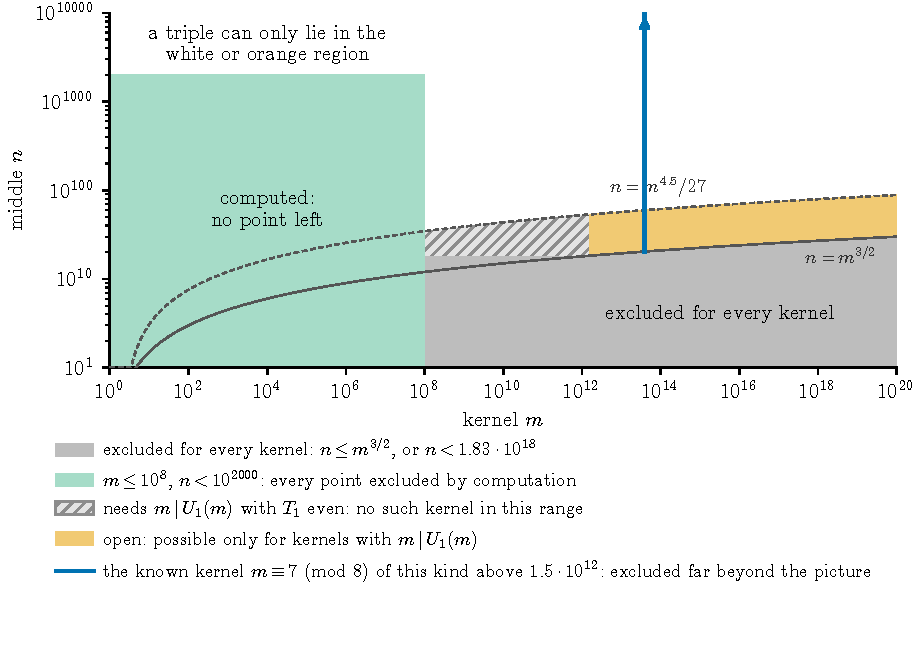
\includegraphics[width=\textwidth]{fig_kartemn}
\caption{\textbf{Where a triple could still lie.} The kernel $m$ on a logarithmic scale, the middle $n$ on a doubly logarithmic one. Gray:
excluded for every kernel, by the height bound of Corollary~\tref{cor:kern} or by Proposition~\tref{prop:paarliste}(d). Hatched: here a middle
needs $m \mid U_1(m)$ with $T_1(m)$ even, and Reinhart's complete list has no such kernel between $\Z{kernschranke}$ and $1.5 \cdot 10^{12}$
(Remark~\tref{rem:reinhartliste}; the parity of $T_1$ is computed in Proposition~\tref{prop:reinhart}). Green: the box of Theorem~\tref{thm:reduktion}, where every lattice point is excluded by computation.
Orange: the weak point of the bound, kernels with $m \mid U_1(m)$ above $1.5 \cdot 10^{12}$ (Question~\tref{q:walsh}); the one known kernel of
this kind above $1.5 \cdot 10^{12}$ in class~$7$ with $T_1$ even, drawn as a line, admits no middle below the height given in
Table~\ref{tab:reinhart}, and so does the other known one, which lies in the box. The picture does not draw the classes of kernels that
Section~\tref{sec:gebiete} excludes, so a triple could lie only in parts of the white and orange regions.}\label{fig:kartemn}
\end{figure}

A positive integer is \emph{powerful} if every prime that divides it divides it at least twice. Erd\H{o}s asked whether three consecutive
integers can all be powerful, and conjectured that they cannot \cite{Erdos1976Manitoba,Bloom364}; on the attribution among Erd\H{o}s's
papers see \cite[Section~7]{BajpaiBennettChan2024}. Mollin and Walsh conjectured it in a form about Pell numbers \cite[p.~111]{MollinWalsh1986a}
(Section~\tref{sec:exponent}). Two consecutive powerful
numbers exist in abundance, since $x^2 - 8y^2 = 1$ has infinitely many solutions, and four consecutive ones are impossible, since one of
four consecutive integers is $2$ modulo $4$. No triple is known. The $abc$ conjecture implies that there are only finitely many, and its
explicit forms give finite bounds (Remark~\tref{rem:abc}); unconditionally the question is open. Bloom records that no triple has a
middle below $7.38 \cdot 10^{28}$ by OEIS A076445 \cite{Bloom364,OEISA076445}, a statement that rests on the listed terms of that sequence
(Section~\tref{sec:daten}).

We expect that there is no triple, and we give the reasons as evidence, not as proof. First, the $abc$ conjecture implies that there are
at most finitely many (Remark~\tref{rem:abc}). Second, none has been found: none has a middle below $\Z{ohnetripelsicher}$
(Proposition~\tref{prop:paarliste}(d)), and none lies below $10^{22}$ by an enumeration of pairs that is described as exhaustive but is
not certified \cite{OEISA060355,MianSiddique2026}. Mian and Siddique prove, with machine-checked theorems in Lean~4, that no triple lies
below $10^{14}$ \cite{MianSiddique2026}; Table~\ref{tab:schranken} lists these bounds with what each rests on. Third, a triple needs a powerful Pell number $T_k(m)$, and this means that for each
divisor $d \ge 5$ of $k$ with $k < d(4d - 1)$ every prime of rank $d$, and there is at least one, must divide $T_d(m)$ at least twice (Corollary~\tref{cor:teiler});
at our \Z{bedpunkte} lattice points the median number of such conditions is \Z{bedmedian} (Proposition~\tref{prop:teilerdaten}). In the
data, a prime $p$ divides the first Pell term that it divides at least twice about as often as the model with probability $1/p$ predicts
(Proposition~\tref{prop:exponenten}); under that model each condition is one more rare event. The third reason is a heuristic, and the
model is not proved.

\begin{table}[ht]
\centering
\small
\begin{tabular}{l p{7.4cm} l}
\hline
no triple below & what the bound rests on & source \\
\hline
$10^{14}$ & machine-checked theorems in Lean~4 & \cite{MianSiddique2026} \\
$\Z{ohnetripelsicher}$ & computation in this part, every witness proved prime, together with Reinhart's computer proof that his list of the
  kernels dividing $U_1$ is complete up to $1.5 \cdot 10^{12}$ & Proposition~\tref{prop:paarliste}(d) \\
$\Z{ohnetripel}$ & the same, if Reinhart's extended search missed nothing & Proposition~\tref{prop:paarliste}(d) \\
$10^{22}$ & an enumeration of the pairs, described as exhaustive, not certified & \cite{OEISA060355,MianSiddique2026} \\
$7.38 \cdot 10^{28}$ & the listed terms of OEIS A076445; the entry does not state that the list is complete & \cite{Bloom364,OEISA076445} \\
\hline
\end{tabular}
\caption{\textbf{Bounds below which no triple of consecutive powerful numbers is known, and what each rests on.} Our two rows and the last one bound the
middle of a triple; the rows for $10^{14}$ and $10^{22}$ are stated for the triple, whose members differ from its middle by at most one.}\label{tab:schranken}
\end{table}

The problem has an exact address system, due to Mollin and Walsh, Walker and Sentance (Lemmas~\tref{lem:kriterium} to~\tref{lem:gerademitte}):
the middle $n$ of a triple is a term $T_k(m)$ of the Pell sequence of a squarefree kernel $m \equiv 7 \pmod 8$, at an odd index $k$ that is
a multiple of the part $m'$ of $m$ prime to $U_1$. So a triple is a lattice point $(m, k)$ at which $T_k(m)$ is even and powerful, and the question
becomes a question about the prime factors of Pell numbers. Two facts make it hard. Granville showed that the nonexistence of triples
implies that there are infinitely many primes $p$ with $p^2 \nmid 2^p - 2$ (Theorem~\tref{cor:wieferich}), a statement that is not known
unconditionally; so a proof would also settle an open problem about Wieferich primes. And an $abc$ inequality with exponent below $4/3$
would exclude all large triples, while the exponents derived from the explicit form of the conjecture, itself unproved, are $1.7$ and more
(Remark~\tref{rem:abc}).

This part does three things. It proves a height inequality that bounds the middle of a triple from below in terms of its kernel, and
splits the kernels into two wings by whether $m$ divides $U_1(m)$. It recasts the reduction of Mollin and Walsh as a statement about
witnesses, primes that divide a Pell number exactly once, and organizes the witnesses by their rank. And it computes: every lattice point
with kernel up to $\Z{kernschranke}$ and $T_k < 10^{\Z{hoehe}}$ is excluded by a certified witness or by parity, and of the \Z{rgpaare}
building blocks $\Prim{d}$ that occur there, \Z{rgzert} are shown not to be powerful by a certified witness, a prime that divides the block exactly once and is proved prime;
\Z{rgoffen} remain open. The weak point of the bound is wing~(ii), the kernels with $m \mid U_1$: for
them only $n > m^{3/2}$ is available, all such kernels up to $1.5 \cdot 10^{12}$ are known \cite[Remark~5.5]{Reinhart2023}, up to
$5.325 \cdot 10^{13}$ with a caveat of the author \cite{Reinhart2024}, and beyond that we know no lower bound for their middles other than
$n > m^{3/2}$ (Section~\tref{sec:hoehe}). Part~II meets the kernels with $m \mid U_1(m)$ and $T_1(m)$ even, of both residue classes, from
the side of pairs, and the collected volume lists the open problems of both parts together.

\paragraph{Main results.}
\begin{itemize}
\item \emph{The height inequality} (Theorem~\tref{thm:hoehe}): at every lattice point,
  \[
    \log_{10} T_k(m) \ \ge\ m'\bigl(1.5 \log_{10} m - \log_{10} m'\bigr) - \log_{10} 2 .
  \]
  With Remark~\tref{rem:siebenundzwanzig}, a triple with middle below $10^H$ has its kernel in one of two wings (Corollary~\tref{cor:fluegel}): $m \nmid U_1$ and
  $m < (27 \cdot 10^H)^{2/9}$, or $m \mid U_1$ and $m < 10^{2H/3}$.
\item \emph{The reduction theorem} (Theorem~\tref{thm:reduktion}): among the \Z{kerne} kernels up to $\Z{kernschranke}$, exactly \Z{punkte}
  lattice points have $T_k < 10^{\Z{hoehe}}$; \Z{paritaetspunkte} of them have $T_k$ odd, and each of the other \Z{zeugenpunkte} has a certified
  witness below $\Z{zeugenschranke}$. So no triple has a middle $n < 10^{\Z{hoehe}}$ with $\operatorname{sqfree}(n^2 - 1) \le \Z{kernschranke}$,
  and no triple at all has a middle below $\Z{ohnetripelsicher}$ (Proposition~\tref{prop:paarliste}(d)).
\item \emph{The witness statement} (Theorem~\tref{thm:zeugen}): there is no triple if and only if every lattice point with $T_1(m)$ even has a witness, and
  a witness can then be found among the primes whose rank divides $k$ with odd cofactor; a powerful $T_k$ would also have to satisfy the
  exponent-$3$ condition of Proposition~\tref{prop:exp3}. The $b$-box (Theorem~\tref{thm:bbox}) excludes every middle, of any size, with
  kernel up to $\Z{bboxkern}$ and squarefree part up to $\Z{bboxb}$; the strip (Theorem~\tref{thm:streifen}) shows that a triple with
  kernel up to $\Z{streifenschranke}$ has a middle of more than $\Z{streifenstellen}$ digits; the smooth kernels (Theorem~\tref{thm:glatt})
  exclude a further range below $10^{\Z{glatthoehe}}$.
\item \emph{The building blocks} (Proposition~\tref{prop:raenge}): of the \Z{rgpaare} primitive parts $\Prim{d}$ on the \Z{rgkerne} kernels of
  the lattice points, \Z{rgzert} have a certified witness; \Z{rgoffen} are open,
  each with at least \Z{offenmin} digits. Theorem~\tref{thm:profil} collects the conditions on a counterexample that this part proves or computes.
\end{itemize}

\paragraph{How to read this part.} Every statement is followed by a paragraph \emph{In words} that says what it means with as few formulas
as possible; a reader who wants the results can read the statements and these paragraphs. A reader who wants to check can read the proofs,
the paragraphs \emph{The computation}, and the tables; every number we computed is generated from the data files of the deposit or from a
cited constant, and every
numbered statement carries a label that says whether it is proved, taken from the literature, computed, measured, a heuristic, or open (see
the table at the end). A statement that combines several kinds carries the label of the part that needs the most trust: a proof that uses our own computation is labeled computed, and a proof that uses a published result is labeled proved. Table~\ref{tab:legende} collects the notation.

\paragraph{Plan.} The rest of this section sets up the notation and the address system. Section~\tref{sec:hoehe} proves the height
inequality and the two wings. Section~\tref{sec:reduktion} states the reduction theorem and describes the computation behind it.
Section~\tref{sec:exponent} proves the exponent condition and the reduction to a witness statement, computes the $b$-box, and records Granville's
theorem. Section~\tref{sec:gebiete} adds the strip, the smooth kernels and the square-type middles. Section~\tref{sec:daten} reports the
data: the exponents at the rank, the list of pairs at distance two, the ladders for the known kernels dividing $U_1$, the witnesses, and the
building blocks. Section~\tref{sec:profil} collects the profile of a counterexample, Section~\tref{sec:routen} records the routes that do
not close the problem, and Section~\tref{sec:fragen} states the open questions.


\subsection{Notation}
A positive integer $n$ is \emph{powerful} if $p^2$ divides $n$ for every prime $p$ that divides $n$.
For a squarefree integer $m \ge 2$ let $\varepsilon_m = T_1 + U_1\sqrt{m}$ be the fundamental solution of $x^2 - m y^2 = 1$,
that is, the solution in positive integers with the smallest $x$. For $k \ge 1$ write
\[
  \varepsilon_m^{\,k} = T_k + U_k\sqrt{m},
\]
and $T_k(m)$, $U_k(m)$ when the kernel $m$ has to be named. Put
\[
  m' = \prod_{p \mid m,\ p \nmid U_1} p,
\]
the product of the primes of $m$ that do not divide $U_1$. For an integer $N \ge 1$ let $\operatorname{sqfree}(N)$ be the product of the
primes that divide $N$ to an odd power.

\inwords A number is powerful when every prime in it appears at least twice; for example $72 = 2^3 \cdot 3^2$ is powerful and $12 = 2^2 \cdot 3$
is not. The equation $x^2 - m y^2 = 1$ is Pell's equation. Its smallest solution $\varepsilon_m$ produces all other solutions as powers, and
$T_k$ and $U_k$ are the two parts of the $k$-th power. The number $m'$ collects the primes of $m$ that do not divide $U_1$.

\subsection{The address system}

\begin{lemma}[Mollin and Walsh {\cite[Theorem, p.~110]{MollinWalsh1986a}}]\tlabel{lem:kriterium}\belegart{literature}
There are three consecutive powerful numbers if and only if there are a squarefree $m \equiv 7 \pmod 8$ and an odd $k$ such that
$T_k(m)$ is an even powerful number and $m$ divides $U_k(m)$. In that case the triple is $(T_k - 1, T_k, T_k + 1)$, and
$m = \operatorname{sqfree}(T_k^2 - 1)$.
\end{lemma}

Mollin and Walsh state the criterion with the fundamental unit of $\mathbb{Q}(\sqrt{m})$. For $m \equiv 7 \pmod 8$ this unit is
$\varepsilon_m$: the ring of integers is $\mathbb{Z}[\sqrt{m}]$, and $m$ has a prime factor $\equiv 3 \pmod 4$, so no unit of norm $-1$ exists.

\inwords The middle $n$ of a triple of consecutive powerful numbers is always even, and it is a Pell number $T_k$ for exactly one kernel $m$.
So the search for triples becomes a search over pairs $(m, k)$.

\begin{lemma}[Walker {\cite[Theorems 2.2(3) and 2.5]{Walker1976}}; Mollin and Walsh {\cite[p.~111]{MollinWalsh1986a}}]\tlabel{lem:walker}\belegart{literature}
Let $m$ be squarefree and let $p$ be a prime dividing $m$. Then $p \mid U_k$ if and only if $p \mid k U_1$. Hence $m \mid U_k$ if and only
if $m' \mid k$.
\end{lemma}

\begin{proof}
By the binomial theorem, $U_k = \sum_{i \text{ odd}} \binom{k}{i} T_1^{k-i} U_1^{\,i} m^{(i-1)/2}$. For $p \mid m$ every term with $i \ge 3$ is
divisible by $p$, so $U_k \equiv k T_1^{k-1} U_1 \pmod p$. From $T_1^2 - m U_1^2 = 1$ we get $T_1^2 \equiv 1 \pmod p$, so $T_1$ is invertible
modulo $p$, and the first claim follows. A prime $p \mid m$ with $p \mid U_1$ divides every $U_k$; a prime $p \mid m$ with $p \nmid U_1$
divides $U_k$ exactly when $p \mid k$. Since $m$ is squarefree, this gives the second claim.
\end{proof}

\inwords Whether $m$ divides $U_k$ depends only on whether $k$ is a multiple of $m'$. So for each kernel the useful indices $k$ are
exactly the multiples of $m'$.

\begin{lemma}[Sentance {\cite[Theorem and Converse, p.~272]{Sentance1981}}]\tlabel{lem:adresse}\belegart{literature}
Let $n \equiv 0 \pmod 4$. Then $n - 1$ and $n + 1$ are both powerful if and only if $n = T_k(m)$ for a squarefree $m \equiv 7 \pmod 8$ and
an odd $k$ with $m' \mid k$.
\end{lemma}

\begin{proof}
($\Leftarrow$) We have $n^2 - 1 = m U_k^2$ and $m \mid U_k$ by Lemma~\tref{lem:walker}, so $n^2 - 1 = m^3 w^2$ for an integer $w$. As $n$ is
even, $n - 1$ and $n + 1$ are coprime, so for every prime $p$ the full power of $p$ in $m^3 w^2$ lies in one of them. Hence each of
$n \pm 1$ has the form $a^3 s^2$ with $a \mid m$ squarefree, and such a number is powerful.
($\Rightarrow$) If $n \pm 1$ are powerful and coprime, then $N = n^2 - 1$ is powerful. Write $N = a^2 b^3$ with $b$ squarefree; then
$N = b (ab)^2$ with $b \mid ab$. So $(n, ab)$ solves $x^2 - b y^2 = 1$, and $(n, ab) = (T_k, U_k)$ for $m = b$ and some $k \ge 1$. From
$n \equiv 0 \pmod 4$ we get $n^2 - 1 \equiv 7 \pmod 8$; as $U_k$ is odd, $m \equiv 7 \pmod 8$. An even $T_k$ forces $k$ odd, since
$T_{2j} = 2T_j^2 - 1$ is odd. Finally $m \mid U_k$ gives $m' \mid k$ by Lemma~\tref{lem:walker}.
\end{proof}

\begin{lemma}[Sentance {\cite[p.~272]{Sentance1981}}; Mollin and Walsh {\cite[Lemma~1.1]{MollinWalsh1986b}}]\tlabel{lem:gerademitte}\belegart{literature}
(General even middle.) Let $n \ge 2$ be even. Then $n - 1$ and $n + 1$ are both powerful if and only if $n = T_k(m)$ for a squarefree odd $m \ge 3$ and an odd $k$
with $m' \mid k$ and $T_1(m)$ even. The pair $(m, k)$ is unique: $m = \operatorname{sqfree}(n^2 - 1)$, and $k$ is determined because $T_k$
increases with $k$. Moreover $m \equiv 7 \pmod 8$ if and only if $n \equiv 0 \pmod 4$, and $m \equiv 3 \pmod 8$ if and only if
$n \equiv 2 \pmod 4$; kernels $m \equiv 1, 5 \pmod 8$ never occur. An odd $n$ never occurs.
\end{lemma}

\begin{proof}
As for Lemma~\tref{lem:adresse}; only the residues change. For $n \equiv 2 \pmod 4$ we get $n^2 - 1 \equiv 3 \pmod 8$, and with $U_k$ odd,
$m \equiv 3 \pmod 8$. For odd $k$ we have $T_k \equiv T_1 \pmod 2$: if $T_1$ is even, every term of
$T_k = \sum_j \binom{k}{2j} T_1^{k-2j} (m U_1^2)^j$ contains a factor $T_1$; if $T_1$ is odd, every term with $j \ge 1$ contains the even
factor $m U_1^2 = T_1^2 - 1$. So $T_k$ is even exactly when $T_1$ is. If $n$ were odd, $n \pm 1$ would be even powerful numbers, hence both
divisible by $4$, which is impossible at distance two.
\end{proof}

The residue split and the uniqueness statement are added here; the rest is Sentance's theorem.

We call a pair $(m, k)$ with $m \equiv 7 \pmod 8$ squarefree and $k$ an odd multiple of $m'$ a \emph{lattice point}. By
Lemma~\tref{lem:adresse}, the lattice points with $T_k$ even are exactly the pairs of powerful numbers at distance two whose middle is
$\equiv 0 \pmod 4$. By Lemma~\tref{lem:kriterium}, a triple needs one more condition: $T_k$ itself must be powerful.

\inwords Two powerful numbers that differ by $2$ always sit around a Pell number $T_k$. So every such pair has an address $(m, k)$, and each
address carries at most one pair. A triple is a pair whose middle is powerful as well. The kernel also tells the remainder: $m \equiv 7
\pmod 8$ exactly when the middle is a multiple of $4$, and $m \equiv 3 \pmod 8$ when it is $2$ more than a multiple of $4$.

\subsection{Notation and terms at a glance}\tlabel{sec:legende}

Table~\ref{tab:legende} collects the symbols and words used in this part, with the place where each is defined.

\begin{table}[ht]
\centering
\small
\begin{tabular}{p{3.2cm} p{8.2cm} l}
\hline
symbol or term & meaning & defined in \\
\hline
powerful & every prime factor occurs at least twice & \S\tref{sec:adresse} \\
$v_p(N)$ & the exponent of the prime $p$ in $N$ & standard \\
$\operatorname{sqfree}(N)$ & the product of the primes that divide $N$ to an odd power & \S\tref{sec:adresse} \\
kernel $m$ & a squarefree $m \ge 2$; for a middle $n$ it is $m = \operatorname{sqfree}(n^2 - 1)$ & Lemma~\tref{lem:gerademitte} \\
$\varepsilon_m$, $T_k$, $U_k$ & the smallest solution $T_1 + U_1\sqrt{m}$ of $x^2 - my^2 = 1$, and its $k$-th power $T_k + U_k\sqrt{m}$
  & \S\tref{sec:adresse} \\
$m'$ & the product of the primes of $m$ that do not divide $U_1$ & \S\tref{sec:adresse} \\
address $(m, k)$ & the pair with $n = T_k(m)$ for a middle $n$ & Lemma~\tref{lem:adresse} \\
lattice point & a pair $(m, k)$ with $m \equiv 7 \pmod 8$ squarefree and $k$ an odd multiple of $m'$ & \S\tref{sec:adresse} \\
wings (i), (ii) & kernels with $m \nmid U_1$, and with $m \mid U_1$ & Corollary~\tref{cor:fluegel} \\
rank $\alpha_m(p)$ & the smallest $k \ge 1$ with $p \mid T_k(m)$ & Lemma~\tref{lem:rang} \\
witness & a prime that divides a number exactly once, which shows that the number is not powerful; the number is mostly $T_k(m)$ or
  $\Prim{d}$ & Theorem~\tref{thm:zeugen} \\
class $7$, class $3$ & kernels $m \equiv 7$, resp.\ $3 \pmod 8$; they belong to middles $n \equiv 0$, resp.\ $2 \pmod 4$
  & Lemma~\tref{lem:gerademitte} \\
$\tau(k)$ & the number of divisors of $k$ & standard \\
$\operatorname{rad}(N)$ & the product of the distinct primes dividing $N$ & standard \\
primitive part $\Prim{d}$, building block & the part of $T_d(m)$ on the primes of rank exactly $d$ & Proposition~\tref{prop:raenge} \\
$\Kreis{n}$ & the $n$-th cyclotomic polynomial & standard \\
Wieferich prime (to base $2$) & a prime $p$ with $p^2 \mid 2^{p-1} - 1$ & standard \\
Wieferich prime for $\varepsilon_m$ & an odd prime $p \nmid m$ with $p^2 \mid T_{\alpha_m(p)}(m)$ & Proposition~\tref{prop:lucaswieferich} \\
$abc$ conjecture & $c < C_\epsilon \operatorname{rad}(abc)^{1 + \epsilon}$ for coprime $a + b = c$ and every $\epsilon > 0$
  & Remark~\tref{rem:abc} \\
certified prime & a prime proved by a deterministic test or by a certificate that a second program checks & Proposition~\tref{prop:raenge} \\
$\psi_{12}$ & the smallest number that passes the strong test to the first twelve prime bases without being prime,
  $318\,665\,857\,834\,031\,151\,167\,461$ \cite{SorensonWebster2017} & Proposition~\tref{prop:raenge} \\
$V_n$ & the Lucas sequence $V_n(2T_1, 1) = 2T_n$ & Proposition~\tref{prop:raenge} \\
$B_1$ & the first-stage bound of the elliptic curve method & Table~\ref{tab:offen} \\
\hline
\end{tabular}
\caption{Symbols and terms of Part I.}\label{tab:legende}
\end{table}

\section{The height inequality}\tlabel{sec:hoehe}

\begin{theorem}[height inequality]\tlabel{thm:hoehe}\belegart{proved}
Let $m \equiv 7 \pmod 8$ be squarefree and let $k$ be an odd multiple of $m'$, so that $m \mid U_k$. Then
\[
  \log_{10} T_k(m) \ \ge\ m' \bigl(1.5 \log_{10} m - \log_{10} m'\bigr) - \log_{10} 2 .
\]
In particular this bound holds for the middle $n = T_k \equiv 0 \pmod 4$ of every pair of powerful numbers at distance two, and so for the
middle of every triple of consecutive powerful numbers.
\end{theorem}

\begin{proof}
Put $d = m/m'$. By definition $d$ divides $U_1$, so $U_1 \ge d$. Hence $T_1 = \sqrt{m U_1^2 + 1} > \sqrt{m}\, U_1 \ge m^{3/2}/m'$. Since
$T_k = (\varepsilon_m^k + \varepsilon_m^{-k})/2 \ge \varepsilon_m^k/2 \ge T_1^k/2$ and $k \ge m'$, we get
$T_k \ge T_1^{m'}/2 > (m^{3/2}/m')^{m'}/2$. Take logarithms.
\end{proof}

\inwords The larger $m'$ is, the larger the middle must be: its number of digits exceeds $m' \log_{10}(m^{1.5}/m') - 1$. This already
forces the middle of any triple with a large $m'$ to be enormous.

We did not find this inequality in the literature. Aktaş and Murty \cite[proof of Theorem~1.3, p.~251]{AktasMurty2017} bound the index
using only the trivial lower bound for the fundamental solution, and Chan \cite[Section~2]{Chan2012} counts solutions of Thue equations; neither uses
that $m'$ divides the index. Mollin and Walsh \cite[p.~111]{MollinWalsh1986a} and Stephens and Williams \cite[p.~619]{StephensWilliams1988}
note that $k$ must be large.

\begin{remark}[the constant in the height bound]\tlabel{rem:siebenundzwanzig}\belegart{proved}
All terms of the binomial expansion $T_k = \sum_j \binom{k}{2j} T_1^{k-2j} (m U_1^2)^j$ are nonnegative, so $T_k \ge T_1^k$. Hence the term
$-\log_{10} 2$ in Theorem~\tref{thm:hoehe} can be dropped:
\[
  T_k \ \ge\ \bigl(m^{3/2}/m'\bigr)^{m'} .
\]
The proof uses only that $m$ is odd and squarefree and that $m' \mid k$. So the same bound holds for kernels $m \equiv 3 \pmod 8$, which
carry the pairs with middle $\equiv 2 \pmod 4$ (Lemma~\tref{lem:gerademitte}).
\end{remark}

\inwords A slightly better bound holds, without the factor $1/2$, and it holds for both kinds of even middles.

\begin{corollary}[kernel bound]\tlabel{cor:kern}\belegart{proved}
Let $m$ and $k$ be as in Theorem~\tref{thm:hoehe}. If $m \nmid U_1$, then $T_k > m^{4.5}/27$. If $m \mid U_1$, then $T_k \ge T_1 > m^{3/2}$.
\end{corollary}

\begin{proof}
If $m \nmid U_1$, then $m' > 1$, and $m'$ is odd, so $m' \ge 3$. By Remark~\tref{rem:siebenundzwanzig},
$\ln T_k \ge f(m')$ with $f(x) = x (1.5 \ln m - \ln x)$. Since $f'(x) = 1.5 \ln m - \ln(e x)$, the function $f$ increases on $[3, m]$ as
soon as $m^{3/2}/e > m$, that is, for $m \ge 8$. As $m' \le m$, we get $\ln T_k \ge f(3) = 4.5 \ln m - 3 \ln 3$, which is the claim. The only
kernel below $8$ is $m = 7$, where $m' = 7$; there the smallest term is $T_7(7) \ge T_1(7)^7 = 8^7$, far above $7^{4.5}/27$.
If $m \mid U_1$, then $U_1 \ge m$, so $T_1 > \sqrt{m}\, U_1 \ge m^{3/2}$, and $T_k \ge T_1$.
\end{proof}

\inwords If $m$ does not divide $U_1$, the middle is larger than $m^{4.5}/27$. If $m$ divides $U_1$, we only know that the middle is
larger than $m^{1.5}$.

\begin{corollary}[two wings]\tlabel{cor:fluegel}\belegart{proved}
Let $H > 0$. Let $n < 10^H$ be the middle of a triple of consecutive powerful numbers, or the middle $n \equiv 0 \pmod 4$ of a pair of
powerful numbers at distance two, and let $m = \operatorname{sqfree}(n^2 - 1)$. Then
\begin{enumerate}
  \item[(i)] either $m \nmid U_1$ and $m < (27 \cdot 10^H)^{2/9}$,
  \item[(ii)] or $m \mid U_1$ and $m < 10^{2H/3}$.
\end{enumerate}
\end{corollary}

\begin{proof}
By Lemmas~\tref{lem:kriterium} and \tref{lem:adresse}, $n = T_k(m)$ for a lattice point $(m, k)$. In case $m \nmid U_1$,
Corollary~\tref{cor:kern} gives $m^{4.5}/27 < n < 10^H$; in case $m \mid U_1$ it gives $m^{3/2} < n < 10^H$.
\end{proof}

\inwords Every triple below $10^H$ has its kernel in one of two ranges. We call them wing~(i), for kernels that do not divide $U_1$, and
wing~(ii), for kernels that do. Wing~(ii) allows much larger kernels.

The condition that separates the wings, $m \mid U_1$ or not, has an exact description by Wieferich primes in number fields, due to Fellini
and Murty \cite[Theorem~1.1]{FelliniMurty2026}. We use only the different height behavior of the two wings.

Wing~(ii) is the weak side. For a kernel with $m \mid U_1$ only the bound $n > m^{3/2}$ of Corollary~\tref{cor:kern} is available. All such
kernels up to $1.5 \cdot 10^{12}$ are known, and up to $5.325 \cdot 10^{13}$ if Reinhart's extended search missed nothing
(Remark~\tref{rem:reinhartliste}); above that we know nothing about their size beyond Corollary~\tref{cor:kern}. A lower bound for $T_1(m)$ that grows faster with $m$ in this class would close this gap, and we do not have one.
Park \cite{Park2012} proves lower bounds for fundamental units that hold for almost all members of certain families. A statement about almost
all members does not exclude a single exception, so it does not close the gap.

\begin{remark}[Reinhart's list]\tlabel{rem:reinhartliste}\belegart{literature}
The squarefree $m$ with $m \mid U_1(m)$ are the members of OEIS A135735 \cite{OEISA135735}. Reinhart proved by computer search that the
list is complete up to $1.5 \cdot 10^{12}$ \cite[Remark~5.5]{Reinhart2023}. His later search covers the squarefree $m$ up to
$5.325 \cdot 10^{13}$ and found four further members, but he writes that he does not claim that these are all the members in that range,
for lack of an independent double check, and that it is likely that all were found \cite[Section~3]{Reinhart2024}. We therefore keep two
bounds apart: below $1.5 \cdot 10^{12}$ the list is complete; below $5.325 \cdot 10^{13}$ it is complete if the extended search missed
nothing. Every statement that uses the larger bound says so. Of the members $m \equiv 7 \pmod 8$, \Z{reinhartsiebensicher} lie below the
smaller bound and \Z{reinhartsieben} below the larger one.
\end{remark}

\inwords A published list of the dangerous kernels exists. Up to $1.5 \cdot 10^{12}$ its author proved it complete. Up to
$5.325 \cdot 10^{13}$ he searched everything, but could not afford a second, independent run, and says so. We keep the two levels apart, and
every statement below names the one it uses.

\section{The reduction theorem}\tlabel{sec:reduktion}

\begin{theorem}[reduction]\tlabel{thm:reduktion}\belegart{computed}
Among the $\Z{kerne}$ squarefree $m \equiv 7 \pmod 8$ with $m \le \Z{kernschranke}$, exactly $\Z{filterfamilien}$ pass the discard criterion
described below, and $\Z{punktfamilien}$ of these have an odd multiple $k$ of $m'$ with $T_k(m) < 10^{\Z{hoehe}}$. Together they have
exactly $\Z{punkte}$ such indices $k$. For $\Z{paritaetspunkte}$ of them $T_k$ is odd. For each of the remaining $\Z{zeugenpunkte}$ there is a
prime $p < \Z{zeugenschranke}$ that divides $T_k$ exactly once. Consequently, there is no triple of consecutive powerful numbers whose
middle $n$ satisfies $n < 10^{\Z{hoehe}}$ and $\operatorname{sqfree}(n^2 - 1) \le \Z{kernschranke}$.
\end{theorem}

\begin{proof}
By Lemma~\tref{lem:kriterium}, such a triple is a lattice point $(m, k)$ with $m \le \Z{kernschranke}$ and $T_k < 10^{\Z{hoehe}}$ at which
$T_k$ is even and powerful. An odd $T_k$ fails the first condition. A prime that divides $T_k$ exactly once shows that $T_k$ is not powerful.
It remains to check that the list of points is complete, which is the computation below.
\end{proof}

\inwords We checked every possible address with a kernel up to $\Z{kernschranke}$ and a middle below $10^{\Z{hoehe}}$. At each of the
$\Z{punkte}$ addresses, either the middle is odd, or a small prime divides it only once. In both cases the middle is not powerful, so no
triple lives there. The theorem says nothing about kernels above $\Z{kernschranke}$ or middles above $10^{\Z{hoehe}}$.

\paragraph{The computation.}
Put $H = \Z{hoehe}$. For each $m \le \Z{kernschranke}$ the continued fraction of $\sqrt{m}$ is computed twice: modulo $m$, which gives
$U_1 \bmod m$ and hence $m'$ by Lemma~\tref{lem:walker}, and in scaled floating point, which gives $\log_{10} T_1$; on a sample of \Z{fpn} kernels, all up to $2 \cdot 10^4$ and the others
drawn at random up to $10^8$, its relative error against the exact value is below $\Z{fpmax}$. A kernel is discarded when $m' > (H + 0.31)/\log_{10} T_1 + 1$. This is rigorous: for every admissible $k$,
$\log_{10} T_k \ge k \log_{10} T_1 - 0.31 \ge m' \log_{10} T_1 - 0.31$, so a discarded kernel has no index with $T_k < 10^H$; the extra $1$
is a margin against rounding. It absorbs any relative error in $\log_{10} T_1$ up to $\log_{10} T_1/(H + 0.31)$, and since $T_1 \ge 4$ for
every $m \equiv 7 \pmod 8$, an error below $3 \cdot 10^{-4}$ is enough, and the measured error is far below that.
For the $\Z{filterfamilien}$ surviving kernels the unit is computed exactly and compared with the modular
route, and the run stops on any mismatch. Each $T_k < 10^H$ is computed exactly and tested for parity and for a prime
$p < \Z{zeugenschranke}$ with $v_p(T_k) = 1$. The discard criterion was also rechecked without floating point, from the bound
$\log_{10} T_1 \ge (\ell - 1)\log_{10}\varphi - \log_{10}\sqrt{5}$, where $\ell$ is the period length of the continued fraction and
$\varphi$ the golden ratio; the numerators of the convergents grow at least like Fibonacci numbers. This was done for a random sample of $\Z{margestich}$ discarded kernels
up to $\Z{margemax}$ and for every discarded kernel up to $\Z{margerand}$: none is contradicted, and the smallest margin by
which a discarded kernel exceeds $10^H$ is $\Z{margemin}$ orders of magnitude. Three versions of the scan, which differ in speed and not in the
criterion, give identical lists of points and witnesses. The list of points with their witnesses is part of the data deposit. Figure~\ref{fig:trichter} shows the numbers.

\begin{figure}[ht]
\centering
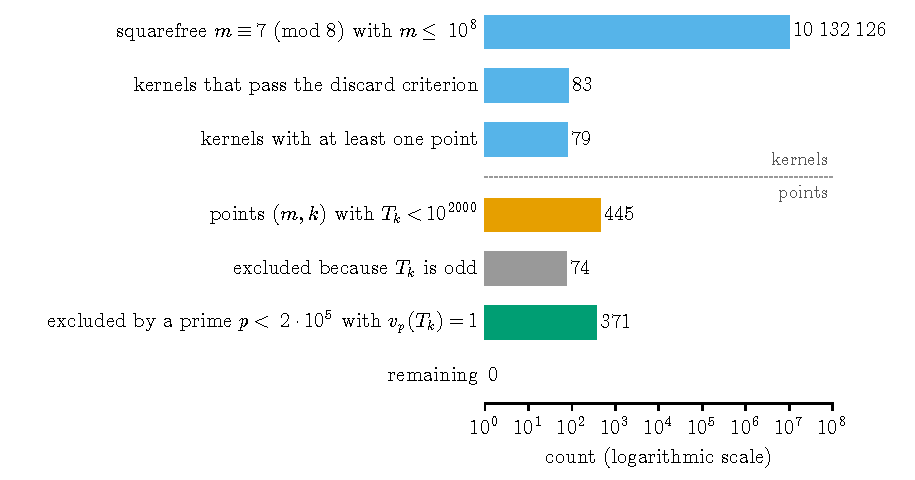
\includegraphics[width=\textwidth]{fig_trichter}
\caption{\textbf{No point of the box remains.} From all kernels to no candidate (Theorem~\tref{thm:reduktion}). The horizontal axis is logarithmic. The upper three bars count
kernels, the lower ones count points $(m, k)$; the two exclusions add up to all points, and none remains.}\label{fig:trichter}
\end{figure}

\paragraph{An example.}
Of the $\Z{punkte}$ points, the one with the smallest middle is $(m, k) = (\Z{beispielm}, \Z{beispielk})$, the example of Mollin and
Walsh \cite[p.~111]{MollinWalsh1986a}. There $\varepsilon_7 = 8 + 3\sqrt{7}$, so $7 \nmid U_1$ and $m' = m$, and
\[
  n = T_{\Z{beispielk}}(\Z{beispielm}) = \Z{beispielwert} = \Z{beispielfaktoren}.
\]
Since $n \equiv 0 \pmod 4$ and $m'$ divides $k$, Lemma~\tref{lem:adresse} shows that $n - 1$ and $n + 1$ are powerful. But the prime
$\Z{beispielzeuge}$ divides $n$ exactly once, so $n$ is not powerful, and $(n - 1, n, n + 1)$ is not a triple. The prime $\Z{beispielzeuge}$ is
the witness recorded for this point.

\begin{remark}[weaker bounds with less work]\tlabel{rem:ohnetripel}\belegart{proved}
The same method gives weaker bounds with less work. The list OEIS A135735 contains all squarefree $m$ with $m \mid U_1(m)$ up to
$1.5 \cdot 10^{12}$, and up to $5.325 \cdot 10^{13}$ if Reinhart's extended search missed nothing (Remark~\tref{rem:reinhartliste}). A
kernel with $m \mid U_1$ that is not on this list is therefore larger than $1.5 \cdot 10^{12}$, and Corollary~\tref{cor:kern} gives
$n > m^{3/2} > \Z{ohnetripelsicher}$ for every triple with such a kernel; under the assumption on the extended search the bound is
$\Z{ohnetripel}$. The
enumeration of consecutive powerful pairs behind the b-file of OEIS A060355 is described by Mian and Siddique as exhaustive below
$10^{22}$ but not certified \cite{OEISA060355,MianSiddique2026}; since every triple contains two such pairs, it excludes triples below that
bound on the same terms. The bound above is stated as Proposition~\tref{prop:paarliste}(d); here it only illustrates the method.
\end{remark}

\inwords A short list plus the height bound already pushes some triples beyond $\Z{ohnetripelsicher}$. This is only an illustration: other searches reach
further, and the reduction theorem is the actual result of this section.

\section{The exponent condition and the witness reduction}\tlabel{sec:exponent}

For a prime $p$ that does not divide $m$, this section describes at which indices $k$ it divides $T_k$, and with which exponent. This
turns the question whether $T_k$ is powerful into a question about finitely many primes.

\begin{lemma}[Bennett and Walsh {\cite[proof of Lemma~3.3, p.~3484]{BennettWalsh1999}}; Lehmer {\cite{Lehmer1930}}]\tlabel{lem:rang}\belegart{literature}
Let $p$ be a prime with $p \nmid m$. Either $p$ divides no $T_k$, or there is a smallest index $\alpha_m(p) \ge 1$ with
$p \mid T_{\alpha_m(p)}$. In the second case, $p \mid T_k$ if and only if $k$ is an odd multiple of $\alpha_m(p)$.
\end{lemma}

We call $\alpha_m(p)$ the \emph{rank} of $p$. Bennett and Walsh state the lemma in the proof of their Lemma~3.3 and characterize the rank in
their Lemma~5.1 \cite[p.~3486]{BennettWalsh1999}, where they call it quite standard and refer to Lehmer.

\inwords A prime appears in the sequence $T_1, T_2, T_3, \ldots$ for the first time at its rank $\alpha$. After that it divides exactly
the terms $T_{\alpha}, T_{3\alpha}, T_{5\alpha}, \ldots$, and no others.

\begin{lemma}[Bennett and Walsh {\cite[Theorem~1.2]{BennettWalsh1999}}]\tlabel{lem:quadratwert}\belegart{literature}
Let $m$ and $b > 1$ be squarefree. There is at most one index $k$ with $T_k = b x^2$ for an integer $x$, and if it exists, then
$k = \alpha_m(b)$, the smallest $k$ with $b \mid T_k$.
\end{lemma}

By Lemma~\tref{lem:rang}, $\alpha_m(b)$ exists if and only if every prime of $b$ has a rank and all these ranks have the same $2$-adic
valuation; then $\alpha_m(b)$ is their least common multiple.

\inwords A term $T_k$ can be $b$ times a square for at most one index $k$, and this index is the first place where $b$ divides the
sequence.

\begin{lemma}[valuation identity]\tlabel{lem:bewertung}\belegart{proved}
Let $p$ be an odd prime with $p \nmid m$ and $p \mid T_r$. Then $v_p(T_{rt}) = v_p(T_r) + v_p(t)$ for every odd $t$.
\end{lemma}

\begin{proof}
Here $v_p(z)$, for $z \in \mathbb{Z}[\sqrt{m}]$, is the largest $e$ with $p^e \mid z$ in $\mathbb{Z}[\sqrt{m}]$, the least $p$-adic valuation of the two
coefficients of $z$. It is not multiplicative when $p$ splits, but it does not change under multiplication by a unit or by an element congruent to $1$ modulo $p$, and
$v_p(tz) = v_p(t) + v_p(z)$ for $t \in \mathbb{Z}$; this is all that the standard proof of the lifting-the-exponent lemma uses.
Put $w = \varepsilon_m^{2r}$ and $u = w + 1 = \varepsilon_m^{r} \cdot 2T_r$, so $v_p(u) = v_p(T_r) \ge 1$. For odd $t$,
\[
  2T_{rt} = \varepsilon_m^{-rt}\,(w^t + 1) = \varepsilon_m^{-rt}\,\bigl(1 - (1 - u)^t\bigr),
\]
and the lifting-the-exponent lemma in $\mathbb{Z}[\sqrt{m}]$ gives $v_p(1 - (1 - u)^t) = v_p(u) + v_p(t)$. It applies because $p$ is odd,
$p \nmid m$, and $p$ divides $u$ but not $1 - u$; the proof is the same as for integers.
\end{proof}

\inwords If a prime $p$ divides $T_r$, then in $T_{rt}$ it appears exactly as often as in $T_r$, plus as often as it divides $t$. So a
prime that appears once in $T_r$ appears once in $T_{rt}$, unless it also divides $t$.

\begin{proposition}[exponent-3 condition]\tlabel{prop:exp3}\belegart{proved}
Let $T_k$ be an even powerful number with $k$ odd and $m' \mid k$, and let $b = \operatorname{sqfree}(T_k)$, so that $T_k = b^3 z^2$ for an
integer $z$. If $b > 1$, then $k = \alpha_m(b)$, and for every odd prime $p \mid b$
\[
  v_p\bigl(T_{\alpha_m(p)}\bigr) + v_p\bigl(\alpha_m(b)/\alpha_m(p)\bigr) \ \ge\ 3 .
\]
\end{proposition}

\begin{proof}
We have $T_k = b (bz)^2$, so $k = \alpha_m(b)$ by Lemma~\tref{lem:quadratwert}. Now let $p \mid b$ be odd. Then $p \mid T_k$, so $k = \alpha_m(p)\, t$ with $t$ odd by
Lemma~\tref{lem:rang}, and $v_p(T_k) = v_p(T_{\alpha_m(p)}) + v_p(t)$ by Lemma~\tref{lem:bewertung}. As $p$ divides the powerful number $T_k$ to an odd power, this power is
at least $3$.
\end{proof}

For general Lucas sequences the valuation identity is standard; see Sanna \cite{Sanna2016}. Ballot \cite[p.~265, (2)]{Ballot2019} printed
it with the term $(\nu - 1) + v_p(n)$, and the errata \cite{Ballot2019Errata} corrects this to $\nu + v_p(n/\rho)$. The corrected form is the
one in Lemma~\tref{lem:bewertung}. On $\Z{ballotfaelle}$ cases of our sequence, the corrected form holds in all of them and the printed form in
$\Z{ballotgedruckt}$; on $\Z{ballotfib}$ cases of the Fibonacci numbers, the corrected form holds in all of them.

\inwords If the middle $T_k$ is powerful, then every prime that divides it an odd number of times divides it at least three times. This
gives a condition on the first term $T_{\alpha(p)}$ in which the prime appears. Proposition~\tref{prop:exp3} does not prove the
conjecture of Mollin and Walsh \cite[p.~111]{MollinWalsh1986a} that $T_k$ is never an even powerful number for odd $k > 1$; it says what
a counterexample would have to satisfy.

\begin{theorem}[the $b$-box]\tlabel{thm:bbox}\belegart{computed}
There is no triple of consecutive powerful numbers whose middle $n$ has kernel $m \le \Z{bboxkern}$ and $\operatorname{sqfree}(n) \le
\Z{bboxb}$, whatever the size of $n$.
\end{theorem}

\begin{proof}
If $\operatorname{sqfree}(n) = 1$, then $n$ is a square, and Theorem~\tref{thm:quadratmitte} gives $m \mid U_1$; no such kernel with $T_1$
even lies below $\Z{bboxkern}$: the kernels $m \mid U_1$ below this bound are listed completely \cite[Remark~5.5]{Reinhart2023}, and the only one with
$m \equiv 7 \pmod 8$, $209\,991$, has $T_1$ odd (Theorem~\tref{thm:quadratmitte}; OEIS \cite{OEISA135735}). Otherwise let $b = \operatorname{sqfree}(n) > 1$ and $n = T_k(m)$. By
Proposition~\tref{prop:exp3}, $k = \alpha_m(b)$, so $\alpha_m(b)$ must exist, be odd and be a multiple of $m'$, and $b^3$ must divide
$T_{\alpha_m(b)}$. We checked all pairs. There are $\Z{bboxfam}$ squarefree $m \equiv 7 \pmod 8$ with $m \le \Z{bboxkern}$; for
$\Z{bboxparitaet}$ of them $T_1$ is odd, so they carry no even middle. The others give $\Z{bboxpaare}$ pairs $(m, b)$ with squarefree
$b \le \Z{bboxb}$, $b = 1$ included. In $\Z{bboxohnealpha}$ pairs some prime of $b$ has no rank, in $\Z{bboxzweiadisch}$ the ranks have different $2$-adic
valuations, in $\Z{bboxkgerade}$ the index $\alpha_m(b)$ is even, and in $\Z{bboxlemmal}$ it is not a multiple of $m'$; this class contains the pairs with $b = 1$, where $k = 1$ while $m' > 1$ for every
such kernel with $T_1$ even \cite{Reinhart2024}. For each of the
remaining $\Z{bboxrest}$ pairs, $b^3$ does not divide $T_{\alpha_m(b)}$; this is tested modulo $b^3$.
\end{proof}

\inwords If the kernel is at most $\Z{bboxkern}$ and the part of the middle with odd exponents is at most $\Z{bboxb}$, there is no triple,
however large the middle is. This result has no height limit, unlike Theorem~\tref{thm:reduktion}.

\begin{theorem}[reduction to a witness statement]\tlabel{thm:zeugen}\belegart{proved}
Let $\mathcal{L}$ be the set of lattice points $(m, k)$ with $T_1(m)$ even. For $(m, k) \in \mathcal{L}$ one has $4 \mid T_k(m)$ and
$\gcd(T_k(m), m) = 1$. The following statements are equivalent.
\begin{enumerate}
  \item[(i)] There are no three consecutive powerful numbers.
  \item[(ii)] For every $(m, k) \in \mathcal{L}$ there is a prime $p$ with $v_p(T_k(m)) = 1$, a \emph{witness}.
  \item[(iii)] For every $(m, k) \in \mathcal{L}$ there is an odd prime $p \nmid m$ such that $k$ is an odd multiple of $\alpha_m(p)$,
  $v_p(T_{\alpha_m(p)}(m)) = 1$, and $p \nmid k/\alpha_m(p)$.
\end{enumerate}
In particular, if $T_k(m)$ is powerful, then $p^2 \mid T_k(m)$ for every prime $p$ with $\alpha_m(p) = k$.
\end{theorem}

\begin{proof}
By Lemmas~\tref{lem:kriterium} and \tref{lem:adresse}, a triple exists if and only if $T_k(m)$ is powerful for some $(m, k) \in \mathcal{L}$.
For every $(m, k) \in \mathcal{L}$ the number $T_k$ is even (proof of Lemma~\tref{lem:gerademitte}), $U_k = m w$ by Lemma~\tref{lem:walker} with
$w$ odd, and $T_k^2 = 1 + m^3 w^2 \equiv 1 + 7 \equiv 0 \pmod 8$, because $m \equiv 7 \pmod 8$; hence $4 \mid T_k$. From $T_k^2 \equiv 1 \pmod m$ we get $\gcd(T_k, m) = 1$. So $T_k$ is powerful if and only if no odd prime $p \nmid m$ has
$v_p(T_k) = 1$, which proves (i)~$\Leftrightarrow$~(ii). For (ii)~$\Leftrightarrow$~(iii): by Lemma~\tref{lem:rang} an odd prime $p \nmid m$
divides $T_k$ exactly when $k$ is an odd multiple of $\alpha_m(p)$, and then $v_p(T_k) = v_p(T_{\alpha_m(p)}) + v_p(k/\alpha_m(p))$ by Lemma~\tref{lem:bewertung}. So $v_p(T_k) = 1$ exactly when $v_p(T_{\alpha_m(p)}) = 1$ and
$p \nmid k/\alpha_m(p)$. For $\alpha_m(p) = k$ the identity reads $v_p(T_k) = v_p(T_{\alpha_m(p)})$, which gives the last claim.
\end{proof}

\inwords Three consecutive powerful numbers do not exist exactly when every address has a witness: a prime that divides the middle
only once. The last sentence says what a counterexample would need. Every prime that appears in $T_k$ for the first time would have to
divide it at least twice, a coincidence of the kind known as a Wieferich condition.

The reduction is due to Mollin and Walsh, who state it and conjecture its conclusion \cite[p.~111]{MollinWalsh1986a}. The mechanism
has a published general form: Fellini and Murty \cite[Lemma~5.6]{FelliniMurty2026} split $\alpha^n - 1$ into a squarefree and a powerful
part in the ring of integers of a number field and show that every prime of the squarefree part is a base-$\alpha$ non-Wieferich prime.
Kym \cite[Corollary~6.6 and Remark~6.7]{Kym2026} gives the closest published form for Lucas sequences: primitive prime divisors in a
coprime product must appear with exponent at least~$2$. Kym studies a different equation and not consecutive powerful numbers. What is
specific here is the translation into the addresses $(m, k)$ and the finite bookkeeping of Section~\tref{sec:daten}.

\begin{lemma}[the $T_1$-part of a lattice point]\tlabel{lem:zweiadisch}\belegart{proved}
Let $m$ be odd and squarefree with $T_1 = T_1(m)$ even, and let $k$ be odd. Then $T_1 \mid T_k$ and $T_k/T_1$ is odd, so
$v_2(T_k) = v_2(T_1)$. For every odd prime $p \mid T_1$ one has $\alpha_m(p) = 1$ and $v_p(T_k) = v_p(T_1) + v_p(k)$. Consequently:
\begin{enumerate}
  \item[(a)] the $2$-adic valuation of the middle of any triple with kernel $m$ is $v_2(T_1(m))$, which is at least $2$ for
  $m \equiv 7 \pmod 8$;
  \item[(b)] if $T_k$ is powerful, then $k$ is divisible by every odd prime $p$ with $v_p(T_1) = 1$.
\end{enumerate}
\end{lemma}

\begin{proof}
We have $T_k = \sum_{j=0}^{(k-1)/2} \binom{k}{2j} T_1^{k-2j} (m U_1^2)^j$, and every term contains $T_1^{k-2j}$ with $k - 2j \ge 1$, so
$T_1 \mid T_k$. In $T_k/T_1$ the term with $j = (k-1)/2$ equals $k (m U_1^2)^{(k-1)/2}$, which is odd because $k$, $m$ and $U_1$ are odd;
$U_1$ is odd since $T_1$ is even and $T_1^2 - m U_1^2 = 1$. Every other term contains $T_1^{k-2j-1}$ with an even exponent at least $2$ and is
even. So $T_k/T_1$ is odd. The $p$-adic formula is the valuation identity of Lemma~\tref{lem:bewertung} with $\alpha_m(p) = 1$. Part~(a)
follows, where $v_2(T_1) \ge 2$ for $m \equiv 7 \pmod 8$ because $T_1^2 = 1 + m U_1^2 \equiv 1 + 7 \equiv 0 \pmod 8$, and part~(b) follows because $v_p(T_k) = 1 + v_p(k) \ge 2$ forces $p \mid k$.
\end{proof}

\inwords All terms $T_k$ with odd $k$ contain $T_1$ as a factor, with the same power of $2$. Every odd prime that divides $T_1$ only once
must also divide the index $k$ of a powerful middle. For $m = 7$ it gives nothing, because $T_1 = 8$; the ladder of Theorem~\tref{thm:streifen} applies the same idea at the index $k_0 = m'$ instead of at $1$, and
for $m = 7$ its first step is the one of Mollin and Walsh.

\begin{corollary}[the divisor count of the Wieferich conditions]\tlabel{cor:teiler}\belegart{proved}
Let $m > 1$ be squarefree and let $k$ be odd. For every divisor $d \ge 5$ of $k$ there is a prime $p_d$ with $\alpha_m(p_d) = d$, and:
\begin{enumerate}
  \item[(i)] every odd prime $p \nmid m$ with $\alpha_m(p) = d$ satisfies $p \equiv \pm 1 \pmod{4d}$, so $p \ge 4d - 1$; in particular no
  prime dividing $d$ has rank $d$;
  \item[(ii)] distinct divisors $d$ give distinct primes $p_d$, and each $p_d$ divides $T_k(m)$; hence the number $\omega(T_k(m))$ of distinct
  prime factors satisfies $\omega(T_k(m)) \ge \#\{d \mid k : d \ge 5\}$, which is $\tau(k) - 1$ if $3 \nmid k$ and $\tau(k) - 2$ if $3 \mid k$;
  \item[(iii)] if $T_k(m)$ is powerful, then for every divisor $d \ge 5$ of $k$ and every prime $p$ with $\alpha_m(p) = d$, in particular for $p_d$, either $p^2 \mid T_d(m)$ or $p \mid k/d$; the second case
  forces $k \ge d(4d - 1)$.
\end{enumerate}
\end{corollary}

\begin{proof}
Put $\alpha = T_1 + U_1\sqrt{m}$ and $\beta = T_1 - U_1\sqrt{m}$. They are the distinct real roots of $z^2 - 2T_1 z + 1$, so
$D_n = (\alpha^n - \beta^n)/(\alpha - \beta) = U_n/U_1$ is a Lucas sequence in the sense of Carmichael, and $D_{2n} = D_n \cdot 2T_n$.
\emph{Existence.} Let $d \ge 5$ divide $k$; then $d$ is odd and $2d \ge 10$. By Carmichael's theorem
\cite{Carmichael1913}, in the form of Yabuta \cite[Theorem~1]{Yabuta2001}, the term $D_{2d}$ has a primitive divisor $p$: $p \mid D_{2d}$ and
$p \nmid D_j$ for $0 < j < 2d$. Since $D_{2d} = D_d \cdot 2T_d$ and $p \nmid D_d$, we get $p \mid 2T_d$; since $p \nmid D_2 = 2T_1$, the prime $p$ is
odd, so $p \mid T_d$. If $p$ divided some $T_j$ with $j < d$, then $p \mid 2T_j \mid D_{2j}$ with $2j < 2d$, which is impossible; so
$\alpha_m(p) = d$. Also $p \nmid m$, because $p \mid m$ would give $T_j^2 = 1 + m U_j^2 \equiv 1 \pmod p$ for all $j$.
\emph{(i)} $p \mid T_d$ means $\varepsilon_m^{2d} \equiv -1 \pmod p$, and $d$ is the smallest index with this property, so $\varepsilon_m$ has
order $4d$ modulo $p$. The elements of norm one in $(\mathbb{F}_p[\sqrt{m}])^\times$ form a cyclic group of order $p - (\tfrac{m}{p})$, and
$\varepsilon_m$ has norm one, so $4d \mid p - (\tfrac{m}{p})$ and $p \equiv \pm 1 \pmod{4d}$. This uses only $\alpha_m(p) = d$, so it holds for
every prime of rank $d$. As $p \ge 4d - 1 > d$, no prime dividing $d$ has rank $d$.
\emph{(ii)} The rank determines $d$, so distinct $d$ give distinct primes. Since $k/d$ is odd, Lemma~\tref{lem:rang} gives $p_d \mid T_k$. The
odd divisors of $k$ below $5$ are $1$ and $3$.
\emph{(iii)} Let $p$ be any prime with $\alpha_m(p) = d$. As above $p \nmid m$, and $p \mid T_k$ as in (ii). If $T_k$ is powerful, then $v_p(T_k) \ge 2$, and
$v_p(T_k) = v_p(T_d) + v_p(k/d)$ by Lemma~\tref{lem:bewertung}. So $p^2 \mid T_d$ or $p \mid k/d$; in the second case $k/d \ge p \ge 4d - 1$ by (i).
The prime $p_d$ is one such prime.
\end{proof}

\inwords Every divisor $d \ge 5$ of $k$ brings its own new prime into $T_k$. For $T_k$ to be powerful, each of these primes must pass a
Wieferich-type test, unless it also divides $k/d$, which forces $k \ge d(4d - 1)$ and is therefore impossible when $d$ is large compared with $\sqrt{k}$. So a counterexample needs many
coincidences at once, each at a different prime; and every further prime of the same rank $d$ must pass the same test. When $k$ is a prime, the count gives only a single condition.

The argument is standard, and it is in print for the Fibonacci and Lucas numbers. The earliest occurrence we found is Luca
\cite[p.~267]{Luca1999}, who derives $\omega(F_n) \ge \tau(n) - 2$ from Carmichael's theorem in the same way. Bugeaud, Luca, Mignotte and
Siksek \cite[proof of Theorem~5]{BugeaudLucaMignotteSiksek2005} use the same step. Pongsriiam \cite[Lemmas~2.5(i) and
3.4(i)]{Pongsriiam2019} states it, including the version for the companion sequence used above, and Somer and K{\v{r}}{\'{\i}}{\v{z}}ek
\cite[Lemma~2.7]{SomerKrizek2015} collect the general facts for Lucas sequences, with the congruence modulo $2n$. What we did not find in
the literature is the statement for the norm-one Pell sequences and the sharpening from modulus $2d$ to modulus $4d$, which follows from
$N(\varepsilon_m) = 1$; neither is a new mechanism. Mollin and Walsh \cite[p.~111]{MollinWalsh1986a} already point to the theory of Lucas
and Lehmer \cite{Lucas1878,Lehmer1930} for this step.

\begin{theorem}[Granville {\cite[Theorem, p.~216]{Granville1986}}]\tlabel{cor:wieferich}\belegart{literature}
If there are no three consecutive powerful numbers, then there are infinitely many primes $p$ with $p^2 \nmid 2^p - 2$.
\end{theorem}

\inwords If triples never exist, then infinitely many primes are not Wieferich primes to base $2$. Nobody knows how to prove this last
statement without extra assumptions. So a proof that triples never exist would also settle an open problem about Wieferich primes.

That infinitely many primes are non-Wieferich is known under the $abc$ conjecture. Silverman \cite[Theorem~1]{Silverman1988} proved it for a fixed
rational base; Kotyada and Muthukrishnan \cite[Theorem~1.1]{KotyadaMuthukrishnan2018} for the fundamental unit of a real quadratic field
of class number one; and Fellini and Murty \cite[Theorem~1.2]{FelliniMurty2026} for number fields, under the $abc$ conjecture of Masser.
Fellini and Murty also derive it from the finiteness of base-$\alpha$ super-Wieferich primes \cite[Theorem~1.3]{FelliniMurty2026}; in the
rational case this is Theorem~1.4 of Murty and S{\'e}guin \cite{MurtySeguin2019}. All of these split $\alpha^n - 1$ into a squarefree and a
powerful part, as this section does. The same splitting, applied to the terms of a Lucas sequence, shows under the $abc$ conjecture that
there are only finitely many powerful terms: Ribenboim and Walsh \cite[Corollary~2]{RibenboimWalsh1999}, and Yabuta \cite[Theorem~2.3]{Yabuta2007}, who
uses the primitive divisor theorem of Bilu, Hanrot and Voutier \cite{BiluHanrotVoutier2001}. For the sequences $T_k(m)$ this gives, under $abc$,
finitely many $k$ for each fixed $m$. The $abc$ conjecture also implies that there are only finitely many triples
\cite[Section~6]{AktasMurty2017}, \cite[Section~1]{Tao2026}. None of these conditional results is effective.

Granville's proof is a construction \cite[pp.~216--217]{Granville1986}. If every prime $p > p_0$ satisfied $p^2 \mid 2^p - 2$, it would
produce a triple whose middle is a power of $2$, and in fact one with middle $A^n$ for every $n \ge 1$, where $A$ is the number of his construction, so that the theorem already holds if there are only
finitely many triples; Granville states it under the conjecture of Mollin and Walsh. In our notation such a middle is $T_k(m) = 2^a$. By Lemma~\tref{lem:zweiadisch} the
number $T_1$ divides $2^a$ and $T_k/T_1$ is odd, so $T_k = T_1$ and $k = 1$. Proposition~\tref{prop:zweierpotenz} treats this case numerically.

\begin{remark}[what the witness condition does not follow from]\tlabel{rem:bouchard}\belegart{proved}
The witness condition does not follow from coprimality. If $n$ and $n + 1$ are powerful, then $\gcd(n, n + 2) \mid 2$ and
$\gcd(n + 1, n + 2) = 1$, so every odd prime factor of $n + 2$ divides neither $n$ nor $n + 1$. This says which primes occur in $n + 2$,
but nothing about their exponents. An example is $n = \Z{bouchardn}$: both $n$ and $n + 1$ are powerful, and
$n + 2 = \Z{bouchardfakt}$, so the new prime $\Z{bouchardp}$ appears twice. If $n$ is even and powerful, then $4 \mid n$, so $n + 2 \equiv 2 \pmod 4$ and $v_2(n + 2) = 1$; this is the reason for the parity filter of
Theorem~\tref{thm:reduktion}, which keeps only kernels with $T_1$ even. The difficulty lies entirely in the case of odd $n$, where the witness must be odd. The step from
``a new prime divides $n + 2$'' to ``some prime divides $n + 2$ exactly once'' is equivalent to the non-existence of a triple, and so, by
Theorem~\tref{thm:zeugen}, to the witness statement (ii) there, which asks for the witness in the middle of a triple instead of in its outer number. An argument of
this shape has been posted \cite{Bouchard2026}; this remark concerns that step and is not an assessment of the preprint.
\end{remark}

\inwords Knowing that a prime is new in $n + 2$ does not tell us how often it appears there. The pair $\Z{bouchardn}$, $\Z{bouchardn} + 1$
shows that a new prime can appear twice in the next number.

\begin{remark}[where a witness in an outer number can sit]\tlabel{rem:aussen}\belegart{proved}
Let $m$ be odd and squarefree with $T_1 = T_1(m)$ even, let $k$ be odd, and let $\gamma$ be a square root of $\varepsilon = T_1 + U_1\sqrt m$
in an extension field, so that $\gamma^{-1}$ is a square root of $\varepsilon^{-1}$. Then $(\gamma \pm \gamma^{-1})^2 = \varepsilon + \varepsilon^{-1} \pm 2 = 2(T_1 \pm 1)$,
and in the same way $(\gamma^k \pm \gamma^{-k})^2 = 2(T_k \pm 1)$. The quotients
\[
V_k = \frac{\gamma^k + \gamma^{-k}}{\gamma + \gamma^{-1}} = \sum_{j=0}^{k-1} (-1)^j \gamma^{\,k-1-2j}, \qquad
W_k = \frac{\gamma^k - \gamma^{-k}}{\gamma - \gamma^{-1}} = \sum_{j=0}^{k-1} \gamma^{\,k-1-2j}
\]
are polynomials with integer coefficients in $(\gamma + \gamma^{-1})^2 = 2(T_1 + 1)$: the terms $j$ and $k - 1 - j$ carry the same sign and
combine to $\gamma^{r} + \gamma^{-r}$ with $r$ even, which is an integer polynomial in $\gamma^2 + \gamma^{-2} = (\gamma + \gamma^{-1})^2 - 2$. Hence
$V_k$ and $W_k$ are integers, and squaring gives
\[
T_k + 1 = (T_1 + 1)\,V_k^2, \qquad T_k - 1 = (T_1 - 1)\,W_k^2 .
\]
Reducing modulo a prime $p \mid T_1 + 1$ amounts to setting $(\gamma + \gamma^{-1})^2 = 0$, that is $\gamma^2 = -1$, where $V_k = k\gamma^{k-1} = \pm k$;
reducing modulo a prime $p \mid T_1 - 1$ amounts to $(\gamma - \gamma^{-1})^2 = 0$, that is $\gamma^2 = 1$, where $W_k = k$. So
$V_k \equiv \pm k \pmod p$ for every prime $p \mid T_1 + 1$, and $W_k \equiv k \pmod p$ for every prime $p \mid T_1 - 1$; all these primes are odd because $T_1$ is even.

Now let $n + 1 = T_k(m)$, so that $n$ and $n + 2$ are the outer numbers. Every prime that divides $n$ or $n + 2$ but not $T_1 \mp 1$ appears
there with an even exponent, so the squarefree parts of the outer numbers are those of $T_1 - 1$ and $T_1 + 1$, whatever $k$ is. An odd prime $q$
divides $n + 2$ exactly once if and only if $q$ divides $T_1 + 1$ exactly once and $q \nmid k$, and likewise for $n$ and $T_1 - 1$; if $q \mid k$,
then $q \mid V_k$ and the exponent is at least $3$. Such a prime divides $m$ and not $U_1$, because $(T_1 - 1)(T_1 + 1) = m U_1^2$ and $q$ divides
exactly one of the two coprime factors, to an odd power; so it divides $m'$. This settles whether the structure forces an odd witness in
$n + 2$ as it forces the prime $2$ when $n$ is even: the candidates are exactly the odd primes that divide $T_1(m) + 1$ exactly once, each of
them is a witness unless it divides $k$, and on a lattice point, where $m' \mid k$ (Lemma~\tref{lem:adresse}), every candidate divides $k$. If
$T_1 + 1$ is a square there is no candidate at all, and $n + 2$ is powerful for every odd $k$. This is the case for every prime kernel
$m \equiv 7 \pmod 8$, by an elementary argument: if $T_1$ were odd, then $U_1$ would be even and the coprime numbers $(T_1 - 1)/2$ and $(T_1 + 1)/2$
would have product $m (U_1/2)^2$, so one of them would be a square $a^2$ and the other $m b^2$ with $b \ge 1$; the case $a^2 - m b^2 = -1$ is
impossible for $m \equiv 3 \pmod 4$, and $a^2 - m b^2 = 1$ would be a solution smaller than the fundamental one. So $T_1$ is even, $T_1 - 1$ and
$T_1 + 1$ are coprime with product $m U_1^2$, one of them is a square, and it is not $T_1 - 1 \equiv 3 \pmod 4$. Hence no odd prime is forced
in the way the prime $2$ is, and for the outer numbers the question returns to Theorem~\tref{thm:zeugen}, which places the witness in the middle.
\end{remark}

\inwords The two neighbors of $T_k$ inherit the primes of odd exponent from the two neighbors of $T_1$; everything else they gain comes in squares. So an odd witness in an outer number can only be a prime of $T_1 \pm 1$, and on a lattice point none of these primes is available.

\begin{remark}[two elementary constraints, and the size of the gap]\tlabel{rem:abc}\belegart{proved}
First, if a prime $q$ divides $N$ and $q > N^{1/2}$, then $v_q(N) = 1$. So a powerful number has no prime factor above its square root, and
a large prime factor is always a witness. Second, $n^2 - (n - 1)(n + 1) = 1$ is an $abc$ equation. For a triple, all three numbers are
powerful, so the radical of $(n - 1)n(n + 1)$ is at most $\bigl((n - 1)n(n + 1)\bigr)^{1/2} < n^{3/2}$, while the largest term is $n^2$.
Hence an $abc$ inequality with exponent below $4/3$ would exclude all large triples. (The $abc$ conjecture states that for every
$\epsilon > 0$ there is a constant $C_\epsilon$ with $c < C_\epsilon \operatorname{rad}(abc)^{1 + \epsilon}$ for all coprime positive
integers with $a + b = c$, where $\operatorname{rad}$ is the product of the distinct prime factors.) The exponents derived from Baker's
explicit form of the conjecture are larger than $4/3$: $7/4$ \cite[Theorem~1]{LaishramShorey2012}, $1.72$ \cite[Theorem~1.4]{ChimShoreySinha2019}, and $1.7$
\cite[Theorem~4.1]{ChimNairShorey2018}; all three assume that explicit conjecture. The explicit form does give a finite bound: under it,
Chim, Shorey and Sinha \cite[Theorem~1.8]{ChimShoreySinha2019} show that the middle of every triple is below $10^{51075}$, and they cite a bound
$10^{20000}$ attributed to Trudgian. Without any hypothesis, the best known bounds in the $abc$ problem are exponential in a power of the
radical \cite{StewartYu2001}.
\end{remark}

\inwords A very large prime factor is always a witness. The $abc$ conjecture in a strong enough form would rule out all large triples.
The explicit forms that have been worked out are themselves conjectures, and they give exponents too large for this. What is proved
without any assumption is much weaker still.

\begin{remark}[the cyclotomic axis]\tlabel{rem:zyklotomisch}\belegart{proved}
If one member of a triple is a proper power $x^r$ with $r \ge 2$, its neighbors are $x^r \pm 1$, and these split into values
$\Kreis{e}(\pm x)$ of cyclotomic polynomials. Each factor gives further conditions on the possible witnesses. These conditions apply only
when a member is a proper power, and they are treated in Part~III. For $r = 2$, the number $x^2 + 1$ is powerful exactly when
$x^2 - b^3 y^2 = -1$ has a solution with $b$ squarefree; this equivalence is due to De Koninck, Doyon and Luca
\cite[(1)--(2)]{DeKoninckDoyonLuca2011}.
\end{remark}

\inwords If one number of a triple is a square, a cube or a higher power, its neighbors split into smaller factors, and each
factor brings its own conditions on a witness. Part~III follows this route.

For a middle that is a cube, four shapes of the neighbors have been excluded, with primes $p$ and $q$: Chan \cite{Chan2025} excludes
$x^3 - 1 = p^3 y^2$ together with $x^3 + 1 = q^3 z^2$, She \cite{She2025} excludes $x^3 - 1 = p^2 a^3$ together with $x^3 + 1 = q^2 b^3$, and
\cite[Theorem~1]{Sayim2026EMW} excludes the two mixed shapes, $x^3 - 1 = p^2 a^3$ with $x^3 + 1 = q^3 z^2$ and $x^3 - 1 = p^3 y^2$ with
$x^3 + 1 = q^2 b^3$. That paper reduces both mixed shapes to the single equation $t^6 + t^3 + 1 = 3w^2$, whose rational solutions it
determines through an elliptic quotient of rank $0$. Each of these results excludes infinitely many candidate middles at once, by an
equation and not by a computation up to a bound.

\section{Exclusion regions and square-type middles}\tlabel{sec:gebiete}

Theorem~\tref{thm:reduktion} covers kernels up to $\Z{kernschranke}$ and middles below $10^{\Z{hoehe}}$. This section adds three results
of a different shape: a strip of small kernels where every possible middle is huge, a box of larger kernels built from small primes, and a
restriction for middles of a special form.

\begin{theorem}[the strip]\tlabel{thm:streifen}\belegart{computed}
There are $\Z{streifenfam}$ squarefree $m \equiv 7 \pmod 8$ with $m \le \Z{streifenschranke}$. For $\Z{streifentot}$ of them $T_1$ is odd,
and no triple has such a kernel. For each of the other $\Z{streifentuerme}$, the middle $n = T_k(m)$ of a triple with kernel $m$ would have
more than $\Z{streifenstellen}$ decimal digits. For $m = 7$ it would have more than $10^{\Z{streifensieben}}$ decimal digits.
\end{theorem}

\begin{proof}
If $T_1$ is odd, then $T_k$ is odd for every odd $k$ (proof of Lemma~\tref{lem:gerademitte}), so $T_k$ is not the middle of a triple.
For the other kernels we climb a ladder of two steps. It rests on Lemma~\tref{lem:rang} and Lemma~\tref{lem:bewertung}: if a prime $p$ divides $T_{k_0}$ exactly once and $k$ is an odd multiple of $k_0$, then
$v_p(T_k) = 1 + v_p(k/k_0)$, so $T_k$ can be powerful only if $p$ divides $k/k_0$. Start with the
smallest admissible index $k_0 = m'$. The primes that divide $T_{k_0}$ exactly once force $k$ to be a multiple of a larger index $k_1$, and
the same argument at $k_1$ gives an index $k_2$. So $T_k \ge T_{k_2}$ whenever $T_k$ can be powerful, and $T_{k_2}$ has the stated number of
digits. In the first run such primes were found at both steps for all but $\Z{streifensteckt}$ kernels; a deeper search found them for
these $\Z{streifensteckt}$ as well, but for $\Z{streifeneins}$ of them only at the first step; there the bound from the first step is already larger
than the smallest one. All other bounds are larger than the smallest one too, which occurs at $m = \Z{streifenminm}$.
\end{proof}

For $m = 7$ the first step is due to Mollin and Walsh \cite[p.~111]{MollinWalsh1986a}: the primes $29$, $197$ and $2857$ divide $T_7(7)$
exactly once, so $k$ must be a multiple of $7 \cdot 29 \cdot 197 \cdot 2857$.

\inwords Of the kernels up to $\Z{streifenschranke}$, the \Z{streifentot} with $T_1$ odd carry no triple at all. For the other
\Z{streifentuerme} a triple is not ruled out, but its middle would be gigantic: it would have more than
$\Z{streifenstellen}$ digits. For $m = 7$ even the number of its digits would be larger than $10^{\Z{streifensieben}}$.

\begin{remark}[the bound of Chim, Shorey and Sinha]\tlabel{rem:chim}\belegart{literature}
Chim, Shorey and Sinha \cite[p.~440]{ChimShoreySinha2019} state the lower bound $10^{3 \cdot 10^{13}}$ for the middle when
$m \in \{15, 23, 31, 39, 47, 55, 87\}$, following the arguments of Mollin and Walsh, and do not give the computation. For $m = 15$, $31$
and $87$ the two-step ladder gives a larger bound, for $m = 23$ and $47$ a smaller one. For $m = 39$ and $55$ the number $T_1$ is odd, so
these kernels carry no triple at all.
\end{remark}

\inwords For the kernels named by Chim, Shorey and Sinha, our ladder gives a larger bound for three and a smaller one for two;
two of them carry no triple at all, because $T_1$ is odd.

\begin{theorem}[smooth kernels]\tlabel{thm:glatt}\belegart{computed}
No triple of consecutive powerful numbers with middle $n < 10^{\Z{glatthoehe}}$ has a kernel $m$ with $\Z{glattunten} < m \le \Z{glattoben}$
whose prime factors are all at most $\Z{glattprim}$ and which has at least $\Z{glattmin}$ prime factors. There are $\Z{glattkerne}$ such
squarefree $m \equiv 7 \pmod 8$. For $\Z{glattgross}$ of them the period $\ell$ of the continued fraction of $\sqrt{m}$ exceeds
$\Z{glattperiode}$, which forces $T_1 > 10^{\Z{glatthoehe}}$. None of the remaining $\Z{glattrest}$ has an admissible index $k$ with
$T_k(m) < 10^{\Z{glatthoehe}}$.
\end{theorem}

\begin{proof}
The numerators $A_j$ of the convergents of $\sqrt{m}$ satisfy $A_j \ge F_{j+2}$, where $F_j$ are the Fibonacci numbers, and $T_1$ is the
numerator at the end of the first period; the period is even because $x^2 - m y^2 = -1$ has no integer solution for $m \equiv 3 \pmod 4$.
So $T_1 \ge F_{\ell + 1} \ge \varphi^{\ell - 1}$, and $\ell > \Z{glattperiode}$ gives
$T_1 > 10^{\Z{glatthoehe}}$. For the other kernels the computation of Theorem~\tref{thm:reduktion} finds no admissible index below
$10^{\Z{glatthoehe}}$.
\end{proof}

\inwords Theorem~\tref{thm:reduktion} stops at kernels up to $\Z{kernschranke}$. For one kind of larger kernel, up to $\Z{glattoben}$ and with all
prime factors at most $\Z{glattprim}$, we can still rule out every triple with a middle below $10^{\Z{glatthoehe}}$. (Such a kernel above
$\Z{glattunten}$ automatically has at least $\Z{glattmin}$ prime factors, since any $\Z{glattmin}$ primes up to $\Z{glattprim}$ have a product below
$\Z{glattunten}$.)

\begin{theorem}[square-type middles]\tlabel{thm:quadratmitte}\belegart{computed}
Let $(n - 1, n, n + 1)$ be a triple of consecutive powerful numbers with $n = T_k(m)$. If $n$ is a square or twice a square, in particular
if $n$ is a fourth power, then $k = 1$ and $m \mid U_1$. Hence either $m > 1.5 \cdot 10^{12}$, or $m$ is one of $209\,991$, $4\,099\,215$
and $117\,477\,414\,815$; if Reinhart's extended search missed nothing (Remark~\tref{rem:reinhartliste}), either $m > 5.325 \cdot 10^{13}$,
or $m$ is one of these three or $39\,028\,039\,587\,479$. None of the four carries a triple with a square-type middle, and $T_1$ is odd for $209\,991$ and
$117\,477\,414\,815$, so that these two kernels carry no triple at all (Lemma~\tref{lem:gerademitte}).
\end{theorem}

\begin{proof}
If $n = X^2$, then $X^4 - m U_k^2 = 1$. By Cohn's theorem \cite{Cohn1997}, quoted as Theorem~1.1 of Bennett and Walsh
\cite{BennettWalsh1999}, the only possible solutions are $X^2 = T_1$ and $X^2 = 2T_1^2 - 1 = T_2$. So $k \in \{1, 2\}$, and $k$ is odd
(Lemma~\tref{lem:kriterium}), so $k = 1$. If $n = 2X^2$, then $T_k = 2X^2$, and by Theorem~1.2 of Bennett and Walsh \cite{BennettWalsh1999}
at most one index $k$ has this property, namely the smallest $k$ with $2 \mid T_k$. As $T_1$ is even for a triple, this is $k = 1$. A fourth
power is a square. In all cases $k = 1$ is a multiple of $m'$, so $m' = 1$ and $m \mid U_1$ by Lemma~\tref{lem:walker}.
The squarefree $m$ with $m \mid U_1(m)$ are listed in OEIS A135735, completely up to $1.5 \cdot 10^{12}$ \cite[Remark~5.5]{Reinhart2023}
and, under the stated assumption, up to $5.325 \cdot 10^{13}$ \cite{Reinhart2024} (Remark~\tref{rem:reinhartliste}); the four values above
are the members with $m \equiv 7 \pmod 8$, the first three below the smaller bound. For $m = 209\,991$ and for $m = 117\,477\,414\,815$ the number $T_1$ is odd
(computed with exact integers), so these two kernels carry no triple at all by Lemma~\tref{lem:gerademitte}. For the
other two, a prime divides $T_1$ exactly once: $\Z{quadratzeuge1}$ for $m = 4\,099\,215$ and $\Z{quadratzeuge3}$ for
$m = 39\,028\,039\,587\,479$. So $n = T_1$ is not powerful.
\end{proof}

Cohn's theorem sharpens Ljunggren's bound of at most two solutions for $x^4 - D y^2 = 1$ \cite{Ljunggren1942a}. Cohn obtains the single
case with two solutions, $D = 1785$, from Ljunggren's result that $y^2 = 2x^4 - 1$ has only the solutions $x = 1$ and $x = 13$
\cite{Ljunggren1942b}.

\inwords If the middle of a triple is a square, twice a square, or a fourth power, then its kernel must divide $U_1$. Such kernels are
known completely up to $1.5 \cdot 10^{12}$, and up to $5.325 \cdot 10^{13}$ if a search that its author could not repeat missed nothing;
none of the known ones carries a triple with such a middle. So a triple of this special shape would need an enormous kernel. The theorem does not exclude these middles; it restricts where they could be.

\begin{remark}[the share of the candidates covered]\tlabel{rem:anteil}\belegart{computed}
Theorem~\tref{thm:quadratmitte} applies to a fixed share of the candidates for a middle. The middle of a triple is powerful and divisible
by $4$ (Lemma~\tref{lem:gerademitte}), so we compare with all powerful $n$ with $4 \mid n$. The number of powerful $n \le x$ is asymptotic to
$(\zeta(3/2)/\zeta(3))\sqrt{x}$ \cite{ErdosSzekeres1934,BatemanGrosswald1958}. The condition $4 \mid n$ multiplies this by
$(\sqrt{2} + 1)/(2\sqrt{2} + 1)$: in the Dirichlet series of the powerful numbers, the Euler factor at $2$ changes from
$1 + 2^{-2s}/(1 - 2^{-s})$ to $2^{-2s}/(1 - 2^{-s})$, and at $s = 1/2$ their quotient is this number. Among these $n$, the squares number
about $\sqrt{x}/2$ and the twice squares about $\sqrt{x}/(2\sqrt{2})$.
Hence, as $x \to \infty$, the share of squares tends to
\[
  \frac{(2\sqrt{2} + 1)\,\zeta(3)}{2(\sqrt{2} + 1)\,\zeta(3/2)} = \Z{mittenquadrat},
\]
the share of twice squares to $\Z{mittendoppel}$, and together to $\Z{mittensatza}$. A count up to $\Z{mittenN}$ gives
$\Z{mittengemessen}$. Cubes and higher odd powers have share tending to $0$.
\end{remark}

\inwords Among all powerful numbers divisible by $4$, which are the candidates for a middle, a little more than three fifths have the
special shape of Theorem~\tref{thm:quadratmitte}. For these, a triple would need a kernel beyond $1.5 \cdot 10^{12}$, and beyond
$5.325 \cdot 10^{13}$ under the assumption of Remark~\tref{rem:reinhartliste}.

\section{Data}\tlabel{sec:daten}

%

\begin{proposition}[exponents at the rank]\tlabel{prop:exponenten}\belegart{measured}
Consider the \Z{expfam} kernels $m \equiv 7 \pmod 8$ with $m \le \Z{expmmax}$ and $T_1(m)$ even, and the primes $3 \le p \le \Z{exppmax}$
that have a rank $\alpha_m(p)$; this gives \Z{exppaare} pairs $(m, p)$. Among them $v_p(T_{\alpha_m(p)}) \ge 2$ holds \Z{expwzwei} times and
$v_p(T_{\alpha_m(p)}) \ge 3$ holds \Z{expwdrei} times. The model in which every pair has $v_p \ge 2$ with probability $1/p$ and $v_p \ge 3$
with probability $1/p^2$, independently, predicts \Z{exphzwei} and \Z{exphdrei}.
\end{proposition}

The model is the usual heuristic for Wieferich primes: Crandall, Dilcher and Pomerance record that the probability that $p$ is a
Wieferich prime to base $2$ is sometimes estimated as about $1/p$ \cite{CrandallDilcherPomerance1997}, and Ryan \cite[Section~1]{Ryan2026}
states it in the same form for the Wieferich locus of an arbitrary algebraic unit, conditional on an equidistribution of Fermat quotients
that is open even for base $2$. In our setting the unit is $\varepsilon_m$ and the event is $p^2 \mid T_{\alpha_m(p)}(m)$, the
Wieferich condition of Proposition~\tref{prop:lucaswieferich}.

Both counts lie within one standard deviation of the prediction. The independence in the model was tested rather than assumed: all
events of one kernel come from the same unit $\varepsilon_m$, so they might cluster. Let $k_m$ be the number of events $v_p \ge 2$ at the
kernel $m$ and $\lambda_m$ the sum of $1/p$ over its pairs. The statistic $S = \sum_m (k_m - \lambda_m)^2$ is \Z{korrs}, against
$\Z{korrmu} \pm \Z{korrsd}$ in \Z{korrreps} simulations of the independent model: $z = \Z{korrz}$, one-sided empirical $p = \Z{korrp}$.
No clustering within kernels is detected. The kernels with $0, 1, 2, 3, 4$ events number \Z{korrvert}. Split by prime, the largest deviation
is $p = \Z{korrmaxp}$ at \Z{korrmaxz} standard deviations, about what testing each prime with an expected count of at least $1$ separately produces by chance; primes with a smaller expected count were not ranked.

The power of the test was measured as well, with data that keep the frequencies of the events but give a common shock to a fraction
$\rho$ of the kernels (\Z{trennlaeufe} runs for each $\rho$). Full coupling, $\rho = 1$, lifts the mean $z$ to about \Z{trennvoll}. At
$\rho = 0.2$ the coupling is detected in \Z{trennzwei}\,\% of the runs, at $\rho = 0.05$ in \Z{trennfuenf}\,\%. So a coupling of strength
$0.2$ or more would very likely have been seen, and a coupling of strength $0.05$ or less cannot be decided from these data.

\inwords For a prime $p$ the chance that $p^2$ divides the first term of the Pell sequence divisible by $p$ should be about $1/p$. Over the
\Z{exppaare} pairs $(m, p)$ this simple rule predicts the observed number of such squares and cubes well. We also checked that the squares do not
come in bunches at single kernels, and we measured how strong a bunching the check would have seen.

\begin{proposition}[no triple below $\Z{ohnetripelsicher}$, and the pairs at distance two with middle divisible by four]\tlabel{prop:paarliste}\belegart{computed}
\begin{enumerate}
\item[(a)] The middles $n \equiv 0 \pmod 4$ of pairs $n - 1$, $n + 1$ of powerful numbers with $n < 10^{\Z{hoehe}}$ and
  $\operatorname{sqfree}(n^2 - 1) \le \Z{kernschranke}$ are exactly the numbers $T_k(m)$ of the \Z{zeugenpunkte} lattice points of
  Theorem~\tref{thm:reduktion} with $T_k$ even.
\item[(b)] Alekseyev's table for OEIS A076445 \cite{OEISA076445} has \Z{alekterme} terms up to its largest, which has \Z{alekstellen} digits.
  Up to that term they are exactly the pairs at distance two of our computation with kernel at most $\Z{klassedreimax}$, for middles
  $\equiv 0$ and $\equiv 2 \pmod 4$ alike. Exactly \Z{alekneun} of them have a middle $\equiv 0 \pmod 4$.
\item[(c)] The list in (a) contains every middle $n \equiv 0 \pmod 4$ of a pair at distance two with $n < \Z{ohnetripelsicher}$, and
  every such middle with $n < \Z{ohnetripel}$ if Reinhart's extended search missed nothing (Remark~\tref{rem:reinhartliste}). It contains
  every such middle with $n < 10^{\Z{vollexpo}}/27$ whose kernel does not divide $U_1$, and every such middle with $n < 10^{\Z{vollexpo}}/27$
  if no squarefree $m \equiv 7 \pmod 8$ with $m \mid U_1(m)$ and $1.5 \cdot 10^{12} < m < 10^{\Z{vollmexpo}}/9$ has
  $T_1(m) < 10^{\Z{vollexpo}}/27$.
\item[(d)] Consequently, with Theorem~\tref{thm:reduktion}, no triple of consecutive powerful numbers has a middle below
  $\Z{ohnetripelsicher}$, and none below $\Z{ohnetripel}$ if Reinhart's extended search missed nothing.
\end{enumerate}
\end{proposition}

\begin{proof}
(a) is Lemma~\tref{lem:adresse} together with the enumeration of Theorem~\tref{thm:reduktion}: a lattice point with $T_k$ odd gives no
middle divisible by four. (b) is a comparison of the two lists; we compared our own values with the table through their hashes, so no
value of the table enters our data. (c) Let $n$ be such a middle and $m$ its kernel. If $m \nmid U_1$, Corollary~\tref{cor:fluegel}(i) gives
$m < (27n)^{2/9}$, which is at most $\Z{kernschranke}$ for $n < 10^{\Z{vollexpo}}/27$. If $m \mid U_1$, part (ii) gives $m < n^{2/3}$ and, since
$n = T_k(m) \ge T_1(m)$, also $T_1(m) \le n$. For $n < \Z{ohnetripelsicher}$ this forces $m < 1.5 \cdot 10^{12}$, the range in which
Reinhart's list of such kernels is complete \cite[Remark~5.5]{Reinhart2023}; its \Z{reinhartsiebensicher} kernels $m \equiv 7 \pmod 8$ all
have $T_1(m) \ge 10^{\Z{reinhartt1}}$, so none of them occurs. For $n < \Z{ohnetripel}$ the same holds with the \Z{reinhartsieben} kernels of
the extended list \cite{Reinhart2024}, if that list is complete (Remark~\tref{rem:reinhartliste}). For $n < 10^{\Z{vollexpo}}/27$ the same
argument leaves exactly the kernels named in the condition. (d) The middle of a triple is such a middle (Lemma~\tref{lem:kriterium}), so by
(c) it is in the list of (a), and every point of that list is excluded in Theorem~\tref{thm:reduktion}.
\end{proof}

\inwords Our list of the middles divisible by four is complete in the box of Theorem~\tref{thm:reduktion}, and it agrees with the longest
published table in both directions. How far it is complete beyond the box depends on the second kind of kernel, the ones dividing $U_1$:
they are known with proof only up to $1.5 \cdot 10^{12}$, which gives completeness up to $\Z{ohnetripelsicher}$ without any assumption, and
up to $\Z{ohnetripel}$ if the extended search missed nothing.

Bloom \cite{Bloom364} states that no triple has a middle below $7.38 \cdot 10^{28}$, by OEIS A076445. This rests on the terms listed
there, and the entry does not state that its list is complete; Mian and Siddique make the same point \cite{MianSiddique2026}.

\begin{proposition}[ladders for the known kernels dividing $U_1$]\tlabel{prop:reinhart}\belegart{computed}
Table~\ref{tab:reinhart} gives, for the two known squarefree kernels $m \equiv 7 \pmod 8$ with $m \mid U_1$ and $T_1(m)$ even, the ladder
of Theorem~\tref{thm:streifen}: at each stage the primes $p \le P$ with $v_p(T_k) = 1$ at the current index $k$, and then the smallest
index a triple with this kernel could still have, together with the number of digits its middle would have at least. The other two known
kernels, $m = \Z{reinhartungerade}$ and $m = \Z{reinhartungerade2}$, have $T_1$ odd (with \Z{reinhartungeradest} and \Z{reinhartungeradest2} digits) and give no
triple by parity.
\end{proposition}

\begin{table}[ht]
\centering
\small
\begin{tabular}{rrr p{4.2cm} rr}
\hline
kernel $m$ & digits of $T_1$ & $P$ & witnesses, stage by stage & $k \ge$ & digits of $n \ge$ \\
\hline
\Z{reinharttab}
\hline
\end{tabular}
\caption{The ladder for the two known kernels $m \equiv 7 \pmod 8$ with $m \mid U_1$ and $T_1(m)$ even. The witnesses of one stage are
separated by commas, the stages by semicolons. The last two columns are rounded down.}\label{tab:reinhart}
\end{table}

\begin{figure}[ht]
\centering
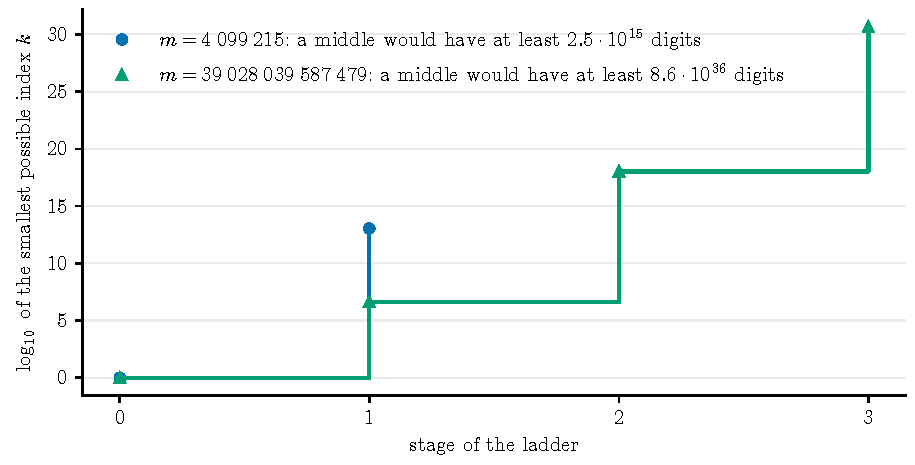
\includegraphics[width=\textwidth]{fig_leiter}
\caption{\textbf{Each stage of a ladder pushes the smallest possible index up.} The ladder of Table~\ref{tab:reinhart}, stage by stage. Each step multiplies the smallest possible index $k$ by the product of
the witnesses of that stage; the last point is the smallest index that remains possible.}\label{fig:leiter}
\end{figure}

\begin{proof}[How the table is computed]
Let $k_0$ be an index with $v_p(T_{k_0}) = 1$ for an odd prime $p$, and let $T_k$ be powerful with $k_0 \mid k$ and $k/k_0$ odd. By
Lemma~\tref{lem:bewertung}, $v_p(T_k) = 1 + v_p(k/k_0) \ge 2$, so $p \mid k/k_0$. Starting at $k_0 = 1$, the product of the witnesses of a
stage therefore divides $k/k_0$, and the next stage starts at $k_0$ times that product. The witnesses are found from $T_1$ and $U_1$
modulo $p^2$, without large integers. The ladder stops at the first stage without a witness below $P$.
\end{proof}

\inwords These two kernels are dangerous in the sense of Section~\tref{sec:hoehe}, because they divide $U_1$; the other two known kernels divide $U_1$ as well, but their $T_1$ is odd. For each of them the table
shows how far out a triple would have to be: the middle would have at least the number of digits in the last column. For
$m = 4\,099\,215$ the indices $k = \Z{reinhartboxk}$ also lie in the box of Theorem~\tref{thm:reduktion}, where they are excluded by the
witnesses \Z{reinhartboxz}.

Reinhart \cite[Def.~1.4, p.~6]{Reinhart2024} asks whether $4\,099\,215$ or $39\,028\,039\,587\,479$, or even $7$, admits an index $k$ with
$T_k$ powerful and $m \mid U_k$ (his condition (C), Question~\tref{q:reinhart}). Our first witnesses $\Z{reinhartza}$ and $\Z{reinhartzc}$ for these two kernels are
his own. The table does not decide the question; it only says how large a positive answer would have to be.

\begin{proposition}[the smallest witnesses]\tlabel{prop:zeugen}\belegart{computed}
For each of the \Z{zeugenalle} lattice points of Theorem~\tref{thm:reduktion} that are excluded by a witness, let $p$ be the smallest
witness and $\alpha_m(p)$ its rank. In \Z{zeugenprim} points the smallest witness is primitive, $\alpha_m(p) = k$; in all others it is a
prime whose rank divides $k$ with odd cofactor. The smallest witness is $29$ in \Z{zeugen29} points, $19$ in \Z{zeugen19}, $11$ in
\Z{zeugen11}, $3$ in \Z{zeugen3}, $5$ in \Z{zeugen5} and $7$ in \Z{zeugen7}; its median is \Z{zeugenmedian} and its maximum
\Z{zeugenmax}. In every point $v_p(T_{\alpha_m(p)}) = 1$ and $p \nmid k/\alpha_m(p)$.
\end{proposition}

The valuation identity of Lemma~\tref{lem:bewertung} was checked in every point. As controls, the point $(\Z{beispielm}, \Z{beispielk})$ has the witness $\Z{beispielzeuge}$ of
rank $\Z{beispielk}$, and the identity predicts $v_{\Z{zeugennkp}}(T_{\Z{zeugennkk}}(7)) = \Z{zeugennkv}$, which the exact computation confirms.

\inwords A triple would have to survive the test of Theorem~\tref{thm:zeugen} not only at the primes that first appear at its index
$k$, but at every small prime whose rank divides $k$. In practice the lattice points fail at small primes: the typical witness is
$19$ or $29$, and only at \Z{zeugenprim} of the points is the smallest witness a prime that first appears at $k$ itself.

\begin{remark}[the condition modulo $36$ and the witnesses]\tlabel{rem:rizzi}\belegart{computed}
By Beckon's condition (Remark~\tref{rem:kongruenzen}) the middle $n$ of a triple satisfies $n \equiv 0$, $8$ or $28 \pmod{36}$; the earliest
derivation we located is Beckon's \cite[Theorem~0.1]{Beckon2019}. Proposition~3(i) of \cite{Sayim2026EMW} refines it to $39$ classes modulo $900$ and
$1209$ classes modulo $44\,100$. Rizzi \cite[Proposition~5.1]{Rizzi2026} derives the condition modulo $36$ again and notes that it agrees with Beckon's; the same
paper reports a search up to $10^{10}$ that finds fourteen pairs and no triple \cite[Chapters~4 and~6]{Rizzi2026}. Of the \Z{zeugenalle} middles of Proposition~\tref{prop:zeugen}, \Z{rizzierfuellt} satisfy the
condition, and the \Z{rizzinicht} that do not are exactly the points whose smallest witness is $3$.
\end{remark}

This is no coincidence. For the middle $n$ of a pair, that is, with $n - 1$ and $n + 1$ powerful, and $4 \mid n$, the condition fails exactly when $n$ is
divisible by $3$ but not by $9$, that is, when
$v_3(T_k) = 1$; then $3$ is a witness, and the smallest one. So the condition modulo $36$ is the case $p = 3$ of the witness reduction.
Since the two computations work by different methods, their agreement on the same points checks both.

\inwords A known rule says what the middle of a triple must look like modulo $36$. Our witness search already contains this rule: the
middles that break it are exactly those where the prime $3$ appears only once.

\begin{proposition}[how many conditions there are, and how often they are met]\tlabel{prop:teilerdaten}\belegart{computed}
\begin{enumerate}
\item[(a)] For the \Z{kongrkerne} kernels of class $7$ with the most lattice points and all primes $p \le \Z{kongrp}$ that have a rank $d$,
  the congruence $p \equiv \pm 1 \pmod{4d}$ of Corollary~\tref{cor:teiler}(i) holds at all \Z{kongrpaare} pairs $(p, d)$.
\item[(b)] Over the \Z{bedpunkte} lattice points of Theorem~\tref{thm:reduktion}, the indices $k$ have \Z{bedteiler} divisors $d \ge 5$ in
  total (median \Z{bedallemedian} per point, maximum \Z{bedallemax}). For \Z{bedausweg} of them (\Z{bedanteil}\,\%) one has $k < d(4d - 1)$,
  so by Corollary~\tref{cor:teiler}(iii) a powerful $T_k$ would need $p_d^2 \mid T_d$ at that $d$. Per point the number of such
  conditions has median \Z{bedmedian}, mean \Z{bedmittel} and maximum \Z{bedmax}.
\item[(c)] For the \Z{beskerne} kernels of class $7$ with the most lattice points (\Z{bespunkte} points), every divisor of every $k$ was
  taken as a rank, and for each rank the first \Z{besnp} primes of that rank below $\Z{besp}$ were tested. Of the \Z{besraenge} rank occurrences (a point together with a divisor of its index, so that $d = 1$ and $d = 3$ are included and one pair $(m, d)$ counts once for every
  point whose index $d$ divides), \Z{besbesetzt} have a prime below this bound, and \Z{beszeuge} of these (\Z{beszeugeant}\,\%) carry a witness; \Z{beswief} carry only
  primes with exponent at least $2$. Testing only the smallest prime of each rank gives \Z{beseinszeuge} of the same \Z{besbesetzt}
  ranks (\Z{beseinsant}\,\%) and \Z{beseinswief} with exponent at least $2$ only.
\end{enumerate}
\end{proposition}

The \Z{besleer} rank occurrences without a prime below the bound are undecided; for $d \ge 5$ they are not known to be free of witnesses, since their smallest prime lies
higher, and among them are the occurrences of $d = 1$ at kernels with $T_1(m)$ a power of $2$, which have no odd prime at all. Parts (b)
and (c) report rates. No proof in this paper depends on them, and Corollary~\tref{cor:teiler} holds independently of them; the single
ranks behind (c) are decided, since one prime of exponent $1$ settles its rank by Theorem~\tref{thm:zeugen}.

\inwords Part (a) checks a proved rule on \Z{kongrpaare} cases. Part (b) counts how many separate tests a triple would have
to pass at a lattice point: typically a few, sometimes a dozen. Part (c) shows how often such a test is actually decided by a small prime:
almost always, and more often when more primes per rank are tried.

\begin{proposition}[middles that are powers of two]\tlabel{prop:zweierpotenz}\belegart{computed}
For every integer $a$ with $2 \le a \le \Z{zweiamax}$, at least one of $2^a - 1$ and $2^a + 1$ is not powerful. In particular no triple has
a middle $2^a$ in this range, that is, a middle of this form with up to \Z{zweistellen} digits.
\end{proposition}

\begin{proof}[The computation]
For each prime $p \le \Z{zweip}$ let $e$ be the order of $2$ modulo $p$. The prime $p$ divides $2^a - 1$ exactly when $e \mid a$, and then
$v_p(2^a - 1) = v_p(2^e - 1) + v_p(a/e)$; so $p$ is a witness for $2^a - 1$ exactly when $e \mid a$, $p^2 \nmid 2^e - 1$ and $p \nmid a/e$.
The prime $p$ divides $2^a + 1$ exactly when $e$ is even and $a$ is an odd multiple of $e/2$, and then $v_p(2^a + 1) = v_p(2^{e/2} + 1) + v_p(2a/e)$; so $p$ is a witness for
$2^a + 1$ exactly when $e$ is even, $a$ is an odd multiple of $e/2$, $p^2 \nmid 2^{e/2} + 1$ and $p \nmid 2a/e$. The loop runs over the
primes rather than over the exponents. Among the \Z{zweiexp} exponents, \Z{zweiminus} (\Z{zweiminusant}\,\%) leave $2^a - 1$ without a
witness below the bound and \Z{zweiplus} (\Z{zweiplusant}\,\%) leave $2^a + 1$ without one; no exponent leaves both without one.
\end{proof}

The exponents without a witness are undecided; they are not known to be powerful: their prime factors lie above the search bound. Equivalently, $2^a - 1$ is
proved not powerful for \Z{zweiminusok} of the exponents and $2^a + 1$ for \Z{zweiplusok}. As controls, the computation of the orders
returns exactly the two Wieferich primes $1093$ and $3511$ below the bound, and $2^3 + 1 = 9$, which is powerful, receives no witness.
Question~\tref{q:zweierpotenz} asks for all $a$.

\inwords If the middle of a triple were a power of two, then $2^a - 1$ and $2^a + 1$ would both be powerful. For every $a$ up to
\Z{zweiamax} a small prime appears exactly once in one of the two numbers. The search runs over primes, which makes it cheap.

%
\begin{figure}[tp]
\centering
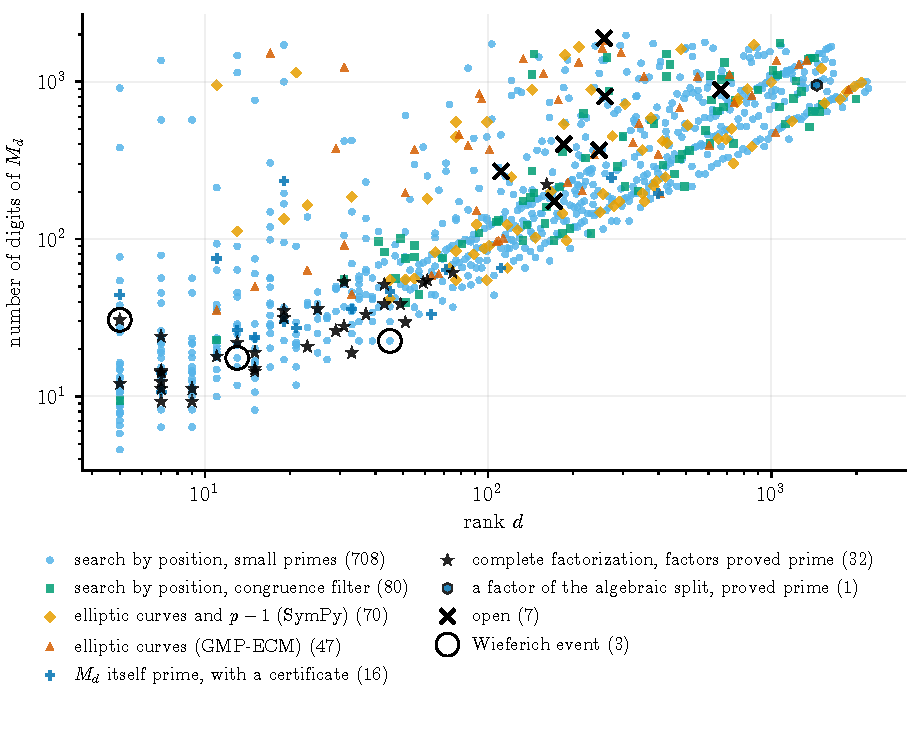
\includegraphics[width=\textwidth]{fig_karte}
\caption{\textbf{Every building block, settled or open.} The \Z{rgpaare} building blocks $\Prim{d}$ of Proposition~\tref{prop:raenge}, one point each: the rank $d$ against the number
of digits, both on logarithmic scales. Color and shape show how each block was shown not to be powerful; the classes are the rows of
Table~\ref{tab:wege}, and every class except the open blocks is a certified witness. The \Z{rgoffen} open blocks (crosses) have at least \Z{offenmin} digits
each, and no search found a factor of them. Circles mark the \Z{wfinpop} blocks with a Wieferich event below $\Z{wfp}$
(Proposition~\tref{prop:lucaswieferich}). The terms are explained in Table~\ref{tab:legende}.}\label{fig:karte}
\end{figure}

\begin{proposition}[the primitive part over an explicit finite set]\tlabel{prop:raenge}\belegart{computed}
Let $\mathcal{P}$ be the set of the \Z{punkte} lattice points of Theorem~\tref{thm:reduktion}; all of them are excluded there. For a
kernel $m$ of a point of $\mathcal{P}$ and an odd $d \ge 5$ dividing an index $k$ with $(m, k) \in \mathcal{P}$, let $\Prim{d}$ be the part of
$T_d(m)$ supported on the primes of rank exactly $d$. There are \Z{rgpaare} such pairs $(m, d)$, on the \Z{rgkerne} kernels of $\mathcal{P}$.
\begin{enumerate}
\item[(a)] \emph{Settled: \Z{rgerledigt} of the \Z{rgpaare}, each by a certified witness.}
\item[(b)] \emph{Open: \Z{rgoffen} of the \Z{rgpaare}.}
\end{enumerate}
\end{proposition}

A witness here is a prime $p$ of rank $d$ with $v_p(\Prim{d}) = 1$; it shows that $\Prim{d}$ is not powerful. For some blocks the witness
comes from a complete factorization, and for one from the algebraic split of Remark~\tref{rem:zweiprimitive}. For a prime $p$ of rank exactly $d$ one has $v_p(\Prim{d}) = v_p(T_d)$ by definition; for the Möbius dual
$\prod_{e \mid d} T_e^{\mu(d/e)}$, the product with which the computations work, the same holds at every prime of rank exactly $d$
\cite[Theorem~2.2(c)]{RossShenCai2026}; the restriction to odd $d$ is the range in which the dual of the
companion sequence is integral \cite[Theorem~2.3]{RossShenCai2026}. Since every point of $\mathcal{P}$ is already excluded, the
proposition excludes no further triple. It asks, on these pairs, whether a primitive part can be powerful
(Question~\tref{q:primindex}). For \Z{rgungerade} of the kernels $T_1(m)$ is odd; their points are excluded by parity alone and enter only
as instances of that question.

\begin{table}[ht]
\centering
\small
\begin{tabular}{lrrr}
\hline
how the pair was settled & first \Z{rgaltkerne} kernels & other \Z{rgneukerne} & all \\
\hline
\Z{wegetab}
\hline
\end{tabular}
\caption{How the \Z{rgpaare} pairs of Proposition~\tref{prop:raenge} were settled. The first \Z{rgaltkerne} kernels are those with the most
lattice points; for the other \Z{rgneukerne}, and for the pairs of the first \Z{rgaltkerne} with $t_{35} < 1$, the elliptic curve method ran to a smaller effort, see Table~\ref{tab:offen}.}\label{tab:wege}
\end{table}

\begin{proof}[How the pairs were settled]
\emph{A search by position.} Every prime $p \le \Z{erstesucheP}$ of rank $d$ was tested, and later, restricted by
Corollary~\tref{cor:teiler}(i) to $p \equiv \pm 1 \pmod{4d}$, every such prime up to $\Z{siebober}$. For the pairs that remain open, this search also shows that no prime of
rank $d$ with $v_p(\Prim{d}) = 1$ lies below its bound.
\emph{A search by size.} The elliptic curve method, first with SymPy \cite{Meurer2017} and then with GMP-ECM \cite{GMPECM706}, looks
for a factor by its size rather than by its position; it shows only what it finds. The effort spent on the pairs that remain open is in
Table~\ref{tab:offen}.
\emph{Complete factorization.} Small primitive parts were factored completely, and some are themselves prime, which no
search for a proper divisor can see. One pair, $(m, d) = (319, 5)$, has no witness below the first bound and
has its own row in Table~\ref{tab:wege}; its witnesses come from the complete factorization of $\Prim{5}(319)$ given after Proposition~\tref{prop:lucaswieferich}, whose large
factors are proved prime.
\emph{Checks.} Every witness was recomputed on a second, independent route (the powers of $\varepsilon_m$ with the rank taken from the
order of the unit, or the Lucas sequence $V_n(2T_1, 1)$, whichever differs from the route that found it). Every witness of the \Z{rgzert} pairs in the first part of (a) is
certified: below $\psi_{12}$ by the Miller--Rabin test with the first twelve prime bases, which is deterministic there
\cite{SorensonWebster2017}, and above it by Pocklington's criterion from a factorization of $p - 1$ \cite[Theorem~4 and Corollary~1]{BrillhartLehmerSelfridge1975},
each certificate checked by a separate program. The prime factors of the complete factorizations and the factor from the algebraic
split are certified in the same way: below $\psi_{12}$ by the deterministic test, and above it \Z{pbpock} of them, with up to
\Z{pbpockmax} digits, by Pocklington's criterion, and \Z{pbecpp}, with up to \Z{pbecppmax} digits, by elliptic curve certificates
\cite{GoldwasserKilian1986,AtkinMorain1993}, which PARI/GP \cite{PARI2172} produced and a separate program of ours checked step by step.
\end{proof}

\begin{table}[ht]
\centering
\small
\begin{tabular}{rrrrrrrr}
\hline
$m$ & $d$ & digits & \multicolumn{3}{c}{curves at $B_1 =$} & $t_{35}$ & $t_{40}$ \\
 & & & $5\cdot 10^4$ & $10^6$ & $3\cdot 10^6$ & & \\
\hline
\Z{offentab}
\hline
\end{tabular}
\caption{The \Z{rgoffen} open pairs of Proposition~\tref{prop:raenge} and the effort of GMP-ECM on each. The columns $t_{35}$ and $t_{40}$
give the fraction of the curves the program expects to need for a factor of $35$ and of $40$ digits, for the second-stage bound it chose.
A fraction of $1$ still misses a factor of that size with probability about $1/e$, so ``none found'' describes the effort, not the
factors. The kernels \Z{offenneum} are among the other \Z{rgneukerne}; the rest are among the first \Z{rgaltkerne}. The blocks that the searches left open on the kernels $m = \Z{teilezeugem}$ and $m = \Z{teilevollm}$, where $T_1(m) + 1$ is a
square, are settled by the algebraic split of Remark~\tref{rem:zweiprimitive} and are not listed.}\label{tab:offen}
\end{table}

\inwords Theorem~\tref{thm:reduktion} already rules out all \Z{punkte} lattice points in its search range. This proposition asks a
different question: can a building block $\Prim{d}$ be powerful at all? We take all \Z{rgkerne} kernels of the lattice points and look at
every building block that occurs there, \Z{rgpaare} in total. A number is powerful when each of its prime factors appears at least twice.
So one prime that appears exactly once is enough to show that a block is not powerful. We found such a prime, and proved that it is
prime, for \Z{rgzert} blocks; for some of them we split the whole block into its prime factors, and for one the algebraic split of
Remark~\tref{rem:zweiprimitive} gives the factor. Every prime used is proved prime, the large ones by certificates that our own program
checks. For the last \Z{rgoffen} blocks we found no such prime. Finding nothing only means that
our search did not succeed, not that no such prime exists.
The \Z{rgoffen} open blocks are in the deposit with their decimal expansions; a prime factor of any one of them with exponent one settles
that block, and a complete factorization settles it either way.

\emph{A different question, measured.} Among the \Z{prtripel} triples $(m, d, p)$ of the search by position with $p \le \Z{erstesucheP}$
(for each rank, the first five primes found by the search), $v_p = 1$ in \Z{prvauf1} cases, $v_p = 2$ in \Z{prvauf2} and $v_p \ge 3$ in none. The heuristic
$P(v_p \ge j) = p^{1-j}$ predicts \Z{prerwartet} triples with $v_p \ge 2$. The observations are consistent with it and do not confirm it.

\begin{remark}[where this stands in the literature]\tlabel{rem:literatur}\belegart{literature}
Ribenboim and Walsh \cite[Corollary~2]{RibenboimWalsh1999} show that the abc conjecture implies that a Lucas sequence of positive discriminant has only
finitely many powerful terms, and Yabuta \cite{Yabuta2007} extends this to negative discriminant. These statements concern the terms rather
than their primitive parts, and they are conditional and not effective, so they neither contain nor are contained in the computation
above. Closer to the question is \cite[Corollary~5.1]{RossShenCai2026}: the primitive parts of the Fibonacci numbers are squarefree for all
$n \ne 6$ if and only if there is no Wall--Sun--Sun prime. Squarefree is a far stronger property than not powerful; the question asked here
is the weaker one, and it is the one a finite computation can address.
\end{remark}

\inwords If the $abc$ conjecture is true, only finitely many terms of such sequences are powerful, but nobody knows which, and the
statement is about whole terms, not their building blocks. For the Fibonacci numbers, even the question whether all building blocks are
squarefree is tied to an open problem about special primes.

\begin{proposition}[Wieferich primes of the unit and the primitive parts]\tlabel{prop:lucaswieferich}\belegart{proved}
Fix a squarefree $m \equiv 7 \pmod 8$ with $T_1(m)$ even. For odd $d \ge 5$ let $\Prim{d}$ be the part of $T_d(m)$ supported on the
primes of rank exactly $d$. Call an odd prime $p \nmid m$ that divides some $T_k(m)$ a \emph{Wieferich prime for $\varepsilon_m$} if
$p^2 \mid T_{\alpha_m(p)}(m)$. The following are equivalent:
\begin{enumerate}
\item[(i)] $\varepsilon_m$ has only finitely many Wieferich primes of odd rank;
\item[(ii)] $\Prim{d}$ is squarefree for all but finitely many odd $d \ge 5$.
\end{enumerate}
In that case $\Prim{d}$ is not powerful for all but finitely many odd $d \ge 5$. Moreover, let $p \nmid m$ be an odd prime that has a rank $\alpha$, let
$u_n = U_n/U_1$ be the Lucas sequence of the first kind for $(P, Q) = (2T_1, 1)$, and let $e = (m/p)$. Then $p \nmid U_1$ and $v_p(u_{p - e}) = v_p(T_\alpha)$.
So the Wieferich primes for $\varepsilon_m$ are exactly the odd Lucas--Wieferich primes of this sequence that divide some $T_k$.
\end{proposition}

\begin{proof}
A prime $p$ dividing $\Prim{d}$ has rank exactly $d$, so $v_p(\Prim{d}) = v_p(T_d) = v_p(T_{\alpha_m(p)})$; in the language of Möbius duals
this is \cite[Theorem~2.2(c)]{RossShenCai2026}. Hence $p$ divides $\Prim{d}$ exactly once when $p$ is not a Wieferich prime for
$\varepsilon_m$. (i) $\Rightarrow$ (ii): a Wieferich prime of odd rank $d$ affects only $\Prim{d}$, so under (i) all $\Prim{d}$ outside
finitely many odd $d$ are squarefree. (ii) $\Rightarrow$ (i): a Wieferich prime of odd rank $d \ge 5$ makes $\Prim{d}$ non-squarefree, so
under (ii) such primes have one of finitely many ranks, and each rank carries finitely many primes, since $\Prim{d}$ is a positive
integer; the ranks $1$ and $3$ carry only the prime divisors of $T_1$ and $T_3$. For the last assertion, $\Prim{d} > 1$ for odd $d \ge 5$,
because $T_d$ has a primitive prime divisor \cite{Carmichael1913}, in the form of \cite{Yabuta2001} used in the proof of
Corollary~\tref{cor:teiler}; and a squarefree integer above $1$ is not powerful.
For the last statement, $p \mid T_\alpha$ gives $\varepsilon_m^{2\alpha} + 1 = 2\varepsilon_m^{\alpha} T_\alpha \equiv 0 \pmod p$ in $\mathbb{Z}[\sqrt{m}]$, and the proof of
Corollary~\tref{cor:teiler}(i) shows that $\varepsilon_m$ has order $4\alpha$ modulo the primes above $p$ and that $4\alpha \mid p - e$; in particular $p \nmid U_1$, because
$p \mid U_1$ would give $\varepsilon_m^2 \equiv 1$. Write $y = \varepsilon_m^{4\alpha}$ and $M = (p - e)/(2\alpha)$, so that $\varepsilon_m^{2(p-e)} = y^M$ and
$y \equiv 1 \pmod p$. Here $p \nmid M$, because $p \nmid p - e$, and $y^M - 1 = (y - 1)(1 + y + \dots + y^{M-1})$ with the second factor congruent to $M$ modulo $p$.
Multiplication by an element of $\mathbb{Z}[\sqrt{m}]$ whose norm is prime to $p$ does not change $v_p$ (see the proof of Lemma~\tref{lem:bewertung}), so
$v_p(y^M - 1) = v_p(y - 1)$. Next, $y - 1 = (\varepsilon_m^{2\alpha} + 1)(\varepsilon_m^{2\alpha} - 1)$ with $\varepsilon_m^{2\alpha} - 1 \equiv -2 \pmod p$ of norm prime to $p$, so
$v_p(y - 1) = v_p(2\varepsilon_m^{\alpha} T_\alpha) = v_p(T_\alpha)$. Finally $\varepsilon_m^{p-e} \cdot u_{p-e} \cdot 2U_1\sqrt{m} = \varepsilon_m^{2(p-e)} - 1$, and the norms of
$\varepsilon_m^{p-e}$ and $2U_1\sqrt{m}$ are prime to $p$, so $v_p(u_{p-e}) = v_p(\varepsilon_m^{2(p-e)} - 1) = v_p(T_\alpha)$.
\end{proof}

\inwords A prime $p$ is a Wieferich prime (to base $2$) if $p^2$ divides $2^{p-1} - 1$. Below $\Z{zweip}$ there are exactly two, $1093$
and $3511$ (the control in Proposition~\tref{prop:zweierpotenz}). Fix one $m$ with $T_1(m)$ even. The rank of a prime $p$ is the first $k$
with $p$ dividing $T_k(m)$. We call $p$ a Wieferich prime for $m$ if $p^2$ already divides the term at its rank. If this rank $d$ is odd and
at least $5$, then $p^2$ divides the block $\Prim{d}$, so $\Prim{d}$ is not squarefree. Proposition~\tref{prop:lucaswieferich} says: the
blocks $\Prim{d}$ with odd $d$ are squarefree from some point on exactly when only finitely many such primes have odd rank. In that case
only finitely many blocks with odd $d$ can be powerful. Such primes do exist. Among the primes below $\Z{wfp}$ we found \Z{wfgerade} of odd
rank $d \ge 5$ on those of the \Z{wfkerne} kernels of Proposition~\tref{prop:raenge} that have $T_1$ even. Since finitely many are allowed, these do not
settle the condition. For \Z{wfentschieden} of them the block is not powerful: another prime divides it exactly once. For the other
\Z{wfoffen} we do not know. Whether a block can be powerful remains open in general. For the Fibonacci numbers, the same kind of
condition is the open question whether a Wall--Sun--Sun prime exists.

For the Fibonacci numbers, Ross, Shen and Cai show that the M\"obius duals $\prod_{d \mid n} F_d^{\mu(n/d)}$ are squarefree for all $n \ne 6$ exactly when there is no
Wall--Sun--Sun prime \cite[Corollary~5.1]{RossShenCai2026}. The proposition is the analog for $\varepsilon_m$, restricted to odd rank
and allowing finitely many exceptions; it is elementary, and its content is the identification of the hypothesis.

\begin{remark}[the Wieferich events of the units]\tlabel{rem:wfdaten}\belegart{computed}
That hypothesis is not empty for our units. Among the primes below $\Z{wfp}$ the \Z{wfkerne} units of Proposition~\tref{prop:raenge} carry \Z{wfereignisse} Wieferich
events, that is, pairs of a unit and a prime (\Z{wfprimzahlen} distinct primes). Of these, \Z{wfungerade} have odd rank $d \ge 5$, and
\Z{wfgerade} of those lie on units with $T_1$ even, where the proposition applies; Table~\ref{tab:wieferich} lists them. So the squarefree
statement for all odd $d$ fails for these units. In \Z{wfzeuge} of the \Z{wfgerade} cases $\Prim{d}$ is nevertheless not powerful, since a
prime of rank $d$ below $\Z{wfp}$ divides it exactly once, and $\Prim{5}(319) = \Z{wfmquadrat}^2 \cdot \Z{wfmgross} \cdot \Z{wfmgroesser}$ with both
large factors proved prime. For the remaining \Z{wfoffen} the question is not settled here; they lie outside the finite set of
Proposition~\tref{prop:raenge}. Conversely, the \Z{wfinpopzu} events whose block lies in that set, the circles in Figure~\ref{fig:karte}, are all
settled; the last column of Table~\ref{tab:wieferich} marks them. On the \Z{erstesuchekerne} units of the first search there are
\Z{wfnullrang} events. Part~III finds more on the same units (Remark~\partref{III}{rem:wieferichbrueche}) because it also counts primes
that divide no $T_k(m)$. Whether a primitive part can be powerful at all is Question~\tref{q:primindex}.
\end{remark}

\begin{table}[ht]
\centering
\begin{tabular}{rrrll}
\hline
unit $m$ & rank $d$ & prime $p$ & $\Prim{d}$ not powerful by & in Prop.~\tref{prop:raenge} \\
\hline
\Z{wftab}
\hline
\end{tabular}
\caption{The Wieferich events of odd rank $d \ge 5$ below $\Z{wfp}$ on the units $\varepsilon_m$ of Proposition~\tref{prop:raenge} with $T_1(m)$ even. ``Witness'': a
prime of rank $d$ below $\Z{wfp}$ divides $\Prim{d}$ exactly once. ``Not settled'': not decided by our computations. The last column says
whether $(m, d)$ is one of the \Z{rgpaare} pairs of Proposition~\tref{prop:raenge}.}\label{tab:wieferich}
\end{table}

\begin{remark}[Lucas--Wieferich primes]\tlabel{rem:lucaswf}\belegart{computed}
The condition in (i) has a name in the computational literature. For the Lucas sequence $(u_n)$ of the first kind attached to $(P, Q) = (2T_1, 1)$,
a prime $p$ with $u_{p - e} \equiv 0 \pmod{p^2}$, where $e$ is the Legendre symbol of the discriminant, is a Lucas--Wieferich prime
\cite[p.~2088]{McIntoshRoettger2007}. That condition is placed on the sequence of the first kind and ours on the companion sequence, but for primes that have a rank the
two agree, by the last statement of Proposition~\tref{prop:lucaswieferich}. The computation agrees as well: on the \Z{lucasgleich} events of the first search of Proposition~\tref{prop:raenge} (the \Z{erstesuchekerne}
units with the most lattice points) the two conditions select the same primes; as controls, the \Z{lucaspk} Wieferich primes $\Z{pellwief}$ of the Pell
sequence are recognized, and \Z{lucasnk} primes that divide their term exactly once are not. This checks the computation on one sequence; the
identity itself is proved above.
\end{remark}

\begin{remark}[a second primitive prime factor]\tlabel{rem:zweiprimitive}\belegart{computed}
If every block $\Prim{d}$ with $d \ge 5$ had two distinct prime factors, a powerful block would need two primes of rank $d$ that each divide
$T_d(m)$ at least twice, two simultaneous events of the kind counted in Proposition~\tref{prop:exponenten}. For Lehmer numbers there is a
theorem of this kind: Juri\v{c}evi\'{c} \cite[Theorems~1.1 and~2.1]{Juricevic2007}, making a result of Schinzel effective, proves that the $n$-th
term of a real Lehmer pair has at least two primitive prime divisors when $n > 4$, $n \ne 6$ and $n/(\eta\kappa)$ is odd, where $\eta$ and $\kappa$ are
invariants of the pair, apart from an explicit list of exceptions with $n \le 30$. Here $\Prim{d}$ is the primitive part of the term of index $2d$ of the Lucas sequence $u_n(2T_1, 1) =
U_n/U_1$, whose terms of even index are $2T_1$ times the Lehmer numbers of the pair with $L = 4T_1^2$ and $M = 1$. For this pair
$\eta = \kappa = 1$, so the condition asks for $2d$ to be odd, and the theorem does not apply to any block.

\emph{A second pair.} If $T_1(m) + 1 = x^2$ is a square, then $\varepsilon = \gamma^2$ with $\gamma + \gamma^{-1} = x\sqrt{2}$, and $(\gamma, \gamma^{-1})$ is a
real Lehmer pair with $L = 2x^2$ and $M = 1$, for which $\kappa = 2$ and $\eta = 2$. Its term of index $4d$ is the term of index $2d$ above, so its
primitive divisors are the primes of rank $d$, and for odd $d \ge 5$ the quotient $4d/(\eta\kappa) = d$ is odd; none of the exceptional triples has
these values. Hence on such a kernel every block $\Prim{d}$ with $d \ge 5$ has at least two distinct prime factors. The split behind it is elementary: for odd $d$,
$T_d + 1 = (x w_d)^2$ with $w_d = (\gamma^d + \gamma^{-d})/(\gamma + \gamma^{-1})$ an integer, so $T_d = (s - 1)(s + 1)$ with $s = x w_d$, and
the odd number $\Prim{d}$ is the product of the coprime factors $\gcd(\Prim{d}, s - 1)$ and $\gcd(\Prim{d}, s + 1)$; that $\Prim{d}$ has two
distinct prime factors is the content of the theorem. This is a splitting of the same kind as the Aurifeuillian factorization of the Lucas numbers,
where the primitive part of $L_{5n}$, for odd $n$, is the product of two coprime factors \cite[(2.9)--(2.11)]{BrillhartMontgomerySilverman1988}.
The case occurs
for \Z{zquadkerne} of the \Z{rgkerne} kernels of Proposition~\tref{prop:raenge}, which carry \Z{zquadbl} of the \Z{rgpaare} blocks, and for every prime kernel
$m \equiv 7 \pmod 8$: the class number is odd, so $x^2 - m y^2 = 2$ is solvable (Remark~\tref{rem:aussen} gives an elementary proof), and we checked it for the \Z{zquadprim} prime kernels below \Z{zquadgrenze}.
We also checked the conclusion on each of these \Z{zquadbl} blocks: $\Prim{d}$ is composite and not a prime power.

On the other kernels the theorem does not apply, and the data show that a block can have a single prime factor: of \Z{zpn} blocks $\Prim{d}$ with $d \ge 5$
and small $T_d(m)$ that we factored completely, \Z{zpprim} are prime, none of them on a kernel of the kind above, the largest at $d = \Z{zpdmax}$, and
\Z{zpab16} of these have $2d \ge 31$, so that it is the parity condition and not the size of $n$ that fails. So on the \Z{zquadkerne} kernels a
powerful block needs two rare events, and on the others no argument of this kind forces two events: a block can have a single prime factor, and a powerful
block could then be the power of a single prime.

The split also settles blocks that the searches of Proposition~\tref{prop:raenge} left open. For $(m, d) = (\Z{teilevollm}, \Z{teilevolld})$
both factors $\gcd(\Prim{d}, s - 1)$ and $\gcd(\Prim{d}, s + 1)$, with \Z{teilevolla} and \Z{teilevollb} digits, are prime, so
$\Prim{d}$ is their product and is not powerful. For $(m, d) = (\Z{teilezeugem}, \Z{teilezeuged})$ one factor, with
\Z{teilezeugest} digits, is prime; since the two factors are coprime, it divides $\Prim{d}$ exactly once. All three primes are proved by
elliptic curve certificates (proof of Proposition~\tref{prop:raenge}).
\end{remark}

\inwords One could hope that a building block always has at least two different primes, so that a powerful block would need two rare
events at once. A theorem of this type exists for a related sequence. On the kernels for which $T_1 + 1$ is a square, it applies after a change of the
sequence, and there every block has at least two primes. On the other kernels its condition is never met by our blocks, and in our data some
blocks are themselves prime. So there one rare event may be all that a powerful block needs.

\section{Profile of a counterexample}\tlabel{sec:profil}

This section collects in one place what is known about a triple, if one exists. Every clause is proved above or computed in
Section~\tref{sec:gebiete} or~\tref{sec:daten}, and the clauses that depend on Reinhart's extended search say so; nothing new is claimed here except clause~(viii).

%
\begin{theorem}[profile]\tlabel{thm:profil}\belegart{computed}
Suppose that $n - 1$, $n$ and $n + 1$ are all powerful, let $m = \operatorname{sqfree}(n^2 - 1)$, and let $(m, k)$ be the address of $n$.
\begin{enumerate}
  \item[(i)] $m \equiv 7 \pmod 8$ is squarefree, $T_1(m)$ is even, $k$ is an odd multiple of $m'$, $n = T_k(m)$, and $4 \mid n$.
  \item[(ii)] $n \ge (m^{3/2}/m')^{m'}$. If $m \nmid U_1$, then $n > m^{9/2}/27$ and $k \ge 3$; if $m \mid U_1$, then $n \ge T_1 > m^{3/2}$.
  \item[(iii)] $v_2(n) = v_2(T_1(m))$, and $k$ is divisible by every odd prime $p$ with $v_p(T_1(m)) = 1$.
  \item[(iv)] Every odd prime $p \mid n$ is coprime to $m$, $k$ is an odd multiple of $\alpha_m(p)$, and
  $v_p(T_{\alpha_m(p)}) + v_p(k/\alpha_m(p)) \ge 2$. Every prime $p$ with $\alpha_m(p) = k$ satisfies $p^2 \mid n$.
  \item[(v)] Let $b = \operatorname{sqfree}(n)$. If $b > 1$, then $k = \alpha_m(b)$, and
  $v_p(T_{\alpha_m(p)}) + v_p(\alpha_m(b)/\alpha_m(p)) \ge 3$ for every odd prime $p \mid b$.
  \item[(vi)] If $n$ is a square, twice a square, or a fourth power, then $k = 1$, $m \mid U_1$, and $m > 1.5 \cdot 10^{12}$ or $m$ is one of
  $209\,991$, $4\,099\,215$ and $117\,477\,414\,815$, which carry no triple with such a middle; if Reinhart's extended search missed nothing
  (Remark~\tref{rem:reinhartliste}), then $m > 5.325 \cdot 10^{13}$ or $m$ is one of the four known values.
  \item[(vii)] Explicit exclusions. Either $m > \Z{kernschranke}$ or $n \ge 10^{\Z{hoehe}}$. If $m \le \Z{bboxkern}$, then
  $\operatorname{sqfree}(n) > \Z{bboxb}$. If $m \le \Z{streifenschranke}$, then $n$ has more than $\Z{streifenstellen}$ digits. If
  $\Z{glattunten} < m \le \Z{glattoben}$ and $m$ is a product of at least $\Z{glattmin}$ primes up to $\Z{glattprim}$, then
  $n \ge 10^{\Z{glatthoehe}}$. If $m \mid U_1$ and $m \le 1.5 \cdot 10^{12}$, then $m = 4\,099\,215$, which
  forces $k \ge \Z{turmk1}$ (the other members of Reinhart's list below this bound, $209\,991$ and $117\,477\,414\,815$, have $T_1$ odd and carry no
  triple); if Reinhart's extended search missed nothing, the same holds for
  $m \le 5.325 \cdot 10^{13}$ with the further kernel $39\,028\,039\,587\,479$ and $k \ge \Z{turmk3}$. In either case $n$ has at least
  $\Z{turmstellen}$ digits. In all cases $n > \Z{ohnetripelsicher}$ (Proposition~\tref{prop:paarliste}(d)).
  \item[(viii)] If $T_1(m) + 1$ is a square, then $n + 1$ is a square. This happens for \Z{zquadkerne} of the \Z{rgkerne} kernels of Proposition~\tref{prop:raenge} and for every
  prime $m \equiv 7 \pmod 8$ (Remark~\tref{rem:zweiprimitive}).
\end{enumerate}
\end{theorem}

\begin{proof}
(i) Lemmas~\tref{lem:kriterium}, \tref{lem:adresse} and \tref{lem:gerademitte}, and Theorem~\tref{thm:zeugen} for $4 \mid n$.
(ii) Remark~\tref{rem:siebenundzwanzig} and Corollary~\tref{cor:kern}; if $m \nmid U_1$ then $m' \ge 3$, so $k \ge 3$.
(iii) Lemma~\tref{lem:zweiadisch}. (iv) Theorem~\tref{thm:zeugen} and Lemma~\tref{lem:bewertung}. (v) Lemma~\tref{lem:quadratwert} and Proposition~\tref{prop:exp3}. (vi) Theorem~\tref{thm:quadratmitte}.
(vii) Theorems~\tref{thm:reduktion}, \tref{thm:bbox}, \tref{thm:streifen} and \tref{thm:glatt}; the kernels $209\,991$ and $\Z{reinhartungerade2}$ have $T_1$ odd
(Theorem~\tref{thm:quadratmitte} and Proposition~\tref{prop:reinhart}), and the bounds for the other two come from the ladder of Theorem~\tref{thm:streifen} applied to these
kernels, as reported in Proposition~\tref{prop:reinhart}. (viii) Remark~\tref{rem:zweiprimitive}: $T_k + 1 = (x w_k)^2$ for odd $k$ if $T_1 + 1 = x^2$.
\end{proof}

\inwords The theorem lists the conditions on a counterexample that this part proves or computes: clauses (i) to (v) are proved, (vi) and (vii) rest on computations. Its kernel $m$ and its index $k$ must pass every test
proved in this paper at the same time: the parity, the height bounds, the exponent conditions, and the explicit searches.

The kernels with $m' = 1$, for which every odd $k$ is admissible, are exactly those with $m \mid U_1$ (Lemma~\tref{lem:walker}); they are
listed in OEIS A135735, completely up to $1.5 \cdot 10^{12}$ \cite[Remark~5.5]{Reinhart2023} and, if Reinhart's extended search missed
nothing, up to $5.325 \cdot 10^{13}$ (Remark~\tref{rem:reinhartliste}). They are the weakest point for an unconditional lower bound on $n$:
an unknown kernel of this kind above $1.5 \cdot 10^{12}$ gives only $n > m^{3/2} > \Z{ohnetripelsicher}$
(the discussion after Corollary~\tref{cor:fluegel} records that no stronger bound is available without hypotheses, and Remark~\tref{rem:abc} discusses the $abc$ route). The enumeration behind the b-file of OEIS A060355
is described by Mian and Siddique as exhaustive below $10^{22}$ but not certified \cite{OEISA060355,MianSiddique2026}. The terms of OEIS A076445 recorded by Bloom reach
$7.38 \cdot 10^{28}$ \cite{Bloom364,OEISA076445}, and Alekseyev's table, which we compare in Proposition~\tref{prop:paarliste}(b), goes up to a term with \Z{alekstellen} digits;
neither list is known to be complete.

\section{Routes that do not close the problem}\tlabel{sec:routen}

Several natural approaches do not decide the problem. This section records why, so that the reasons are available together.

\begin{remark}[congruences]\tlabel{rem:kongruenzen}\belegart{literature}
Beckon \cite[Theorem~0.1]{Beckon2019} showed that the smallest member $n$ of a triple $(n, n + 1, n + 2)$ of powerful numbers satisfies
$n \bmod 36 \in \{7, 27, 35\}$. Proposition~3 of \cite{Sayim2026EMW} refines this: modulo $\ell^2$ the proportion of admissible residues is
$1/4$ for $\ell = 2$, $1/3$ for $\ell = 3$ and $(\ell^2 - 3\ell + 3)/\ell^2$ for $\ell \ge 5$, and the density of admissible residues tends
to $0$ like $(\log L)^{-3}$. Every factor is positive, so for every finite modulus some residue class survives, and no finite sieve of this type decides the problem.
Over the primes up to $\Z{kongruenzbis}$ the product of these proportions is about $\Z{kongruenzdichte}$. Congruences
remain useful as search filters: by Corollary~\tref{cor:teiler}(i), a prime of rank $d$ satisfies $p \equiv \pm 1 \pmod{4d}$, so a search for
such primes needs only $2$ of the $2d$ odd residue classes modulo $4d$.
\end{remark}

\inwords Conditions modulo a fixed number can never rule out all triples: some remainders always survive. They thin out the candidates
more and more, but never to zero. They are still good filters for computer searches.

\begin{remark}[Yokoi's representation]\tlabel{rem:yokoi}\belegart{computed}
Mollin and Walsh \cite[p.~112]{MollinWalsh1986a} suggest that Yokoi's representation of the fundamental unit \cite[Proposition~1]{Yokoi1970}
may help. In our notation it gives, for a prime $p \equiv 3 \pmod 4$ dividing both $m$ and $U_1$, that $p^2$ divides $T_1 - 1$ or $T_1 + 1$.
The identity $T_1^2 - 1 = m U_1^2$ gives more: $p^3$ divides $(T_1 - 1)(T_1 + 1)$, and since $p$ is odd, $p^3$ divides one of the two
factors. So the representation adds no new constraint. We checked this on all $\Z{yokoipaare}$ such pairs $(m, p)$ with $T_1$ even and
$m \le \Z{yokoimax}$.
\end{remark}

\inwords An idea that Mollin and Walsh suggested gives nothing new here: the condition it yields already follows from the equation
$T_1^2 - 1 = m U_1^2$.

\begin{remark}[small units]\tlabel{rem:designa}\belegart{computed}
A search beyond Theorem~\tref{thm:reduktion} might target kernels with a small fundamental unit, where many indices fit below a height
bound. The kernels $m = t^2 - 2$ with $t$ odd and $m = t^2 - 1$ with $4 \mid t$ have the units $(t^2 - 1) + t\sqrt{m}$ and $t + \sqrt{m}$.
There $U_1 = t$ with $t$ odd, resp.\ $U_1 = 1$, is prime to $m$, so $m' = m$, and by Theorem~\tref{thm:hoehe} the first admissible index $k = m$ is already far out. Among the
$\Z{designkerne}$ such squarefree kernels $m \equiv 7 \pmod 8$ with $t \le \Z{designtmax}$, only $\Z{designfenster}$ have a first candidate
$T_{m}(m)$ with fewer than $\Z{designstellen}$ digits, and all of them have $m \le \Z{designmaxm}$, inside the range of
Theorem~\tref{thm:reduktion}. For these two kinds of kernel, small units therefore bring no new kernels into reach.
\end{remark}

\inwords A small unit sounds helpful, but it makes $m'$ as large as $m$, and then the first possible middle is enormous. For the two
kinds of kernel we checked, nothing new appears.

The route through the $abc$ conjecture is discussed in Remark~\tref{rem:abc}: the uniform explicit exponents are too weak, and the full
explicit form gives only a conditional bound.

\begin{remark}[the polynomial analog]\tlabel{rem:polynom}\belegart{literature}
Over the polynomials in one variable over a field of characteristic $0$, not even two consecutive nonconstant powerful polynomials exist.
If $f$ and $f + 1$ are both powerful of degree $n \ge 1$, the theorem of Mason and Stothers \cite{Stothers1981,Mason1984}, applied to
$(f + 1) - f = 1$, gives $n \le \deg \operatorname{rad}\bigl(f(f + 1)\bigr) - 1 \le n/2 + n/2 - 1$, a contradiction; see Snyder
\cite{Snyder2000} for a short proof of the theorem. In the integers there are infinitely many consecutive powerful pairs, such as $(8, 9)$
and $(288, 289)$ \cite{Golomb1970}. The proof uses the derivative, which has no analog for integers. In characteristic $p$ the statement
fails as well: $x^p$ and $x^p + 1 = (x + 1)^p$ are consecutive $p$-th powers, because the derivative of a $p$-th power vanishes.
\end{remark}

\inwords For polynomials the problem is easy, even for pairs, because one can take derivatives. For whole numbers there is no derivative,
and pairs of consecutive powerful numbers do exist. So the polynomial proof cannot be copied.

\section{Open questions}\tlabel{sec:fragen}

\begin{question}[finiteness of the kernels of wing (ii)]\tlabel{q:walsh}\belegart{open}
Are there only finitely many squarefree $m \equiv 7 \pmod 8$ with $m \mid U_1(m)$ and $T_1(m)$ even?
\end{question}

These are the kernels of wing~(ii) in Corollary~\tref{cor:fluegel}, the weakest point for an unconditional bound
(Section~\tref{sec:profil}). Walsh \cite[p.~97]{Walsh1988} asks the corresponding question for all squarefree $m$ with $m \mid U_1(m)$.

\begin{question}[the primitive part of $T_d(m)$]\tlabel{q:primindex}\belegart{open}
Let $m \equiv 7 \pmod 8$ be squarefree with $T_1(m)$ even, let $d \ge 5$ be odd, and let $\Prim{d}$ be the part of $T_d(m)$ supported on the primes of rank exactly $d$. Can $\Prim{d}$ be powerful?
\end{question}

The case of a prime $d$ is, in our view, the hardest, since Corollary~\tref{cor:teiler} then gives a single condition. Section~\tref{sec:daten} examines
the question on a finite set of pairs $(m, d)$. For the Fibonacci numbers, Fathi \cite[Theorems~1.2--1.6]{Fathi2026} shows for several infinite families of
indices $n$, among them every prime power $n > 2$, that $F_n$ has a prime factor that first appears at $n$ and occurs to an odd power. For
these $n$ the primitive part is not a square; this is weaker than not being powerful. Granville \cite[Theorem~3]{Granville2012}
proves, for recurrences $x_{n+2} = b\,x_{n+1} + c\,x_n$ with $c \equiv 2 \pmod 4$ and further conditions, that the terms have a primitive
prime factor to an odd power. Our recurrence $T_{n+2} = 2T_1 T_{n+1} - T_n$ has $c = -1$, and the question here asks for exponent one, not
for an odd exponent.

\begin{question}[a middle that is a power of $2$]\tlabel{q:zweierpotenz}\belegart{open}
Can $2^a - 1$ and $2^a + 1$ both be powerful for some $a \ge 2$?
\end{question}

This is the case of a middle that is a power of $2$, the case that Granville's construction produces (Section~\tref{sec:exponent}).
Proposition~\tref{prop:zweierpotenz} answers it for all exponents up to a bound. She \cite[p.~7]{She2025} conjectures that $x^n - 1$ is never powerful
for $x > 1$ and $n > 2$, which would answer the question.

\begin{question}[Reinhart's condition (C)]\tlabel{q:reinhart}\belegart{open}
Does Reinhart's condition~(C) \cite[Definition~1.4]{Reinhart2024} hold for some squarefree $d$, that is, is there an index $k$ with
$T_k(d)$ powerful and $d \mid U_k(d)$? For $d \mid U_1(d)$ the second condition holds for every $k$.
\end{question}

Reinhart asks this in particular for $d = 4\,099\,215$ and $d = 39\,028\,039\,587\,479$, and even for $d = 7$ \cite[p.~6]{Reinhart2024}. For
odd $k$, Theorems~\tref{thm:streifen} and \tref{thm:profil}(vii) show how large such an index would have to be.

\emph{An expectation of the author, not a claim.} If a triple exists, we expect it to belong to a special case that is singled out by an
additional equation, such as a middle that is a proper power, rather than to a lattice point without such structure. The reason is the
model of Proposition~\tref{prop:exponenten}: at a point without additional structure every condition of Corollary~\tref{cor:teiler} is one
more rare event, so a triple there would need many independent coincidences, while an algebraic identity can satisfy several conditions
at once, as the Pell equations do for pairs. The special shapes treated so far, the cube middles of \cite{Chan2025,She2025,Sayim2026EMW},
the square-type middles of Theorem~\tref{thm:quadratmitte} and the powers of $2$ of Proposition~\tref{prop:zweierpotenz}, are excluded or
restricted. The expectation says where a triple would most likely be found, not whether one exists.

\inwords These are the questions this part leaves open. The first asks whether the dangerous kernels of wing~(ii) are finite in number.
The second asks whether a building block of the middle can be powerful. The third asks whether the middle can be a power of $2$,
which Proposition~\tref{prop:zweierpotenz} rules out for small exponents. The fourth is Reinhart's question for single kernels, including
the three of Table~\ref{tab:reinhart}. Whether the structure forces an odd witness in an outer number is settled by Remark~\tref{rem:aussen}: it does not, beyond the primes of $T_1 \pm 1$.

\section*{The type of every statement}

Every statement of this part carries one of six labels, printed after its number. The table lists them; it is generated from the text by the build and checked against a second, independent reading of the source.

\input{../gemeinsam/belegtab_\teilnr}

%
%
%
%
%
\section*{Data and code availability}\addcontentsline{toc}{section}{Data and code availability}

Every number of this \ifimband volume\else part\fi\ that we computed is generated from a result file of a data deposit or from a cited constant; no computed number is
typed by hand. The data deposit is archived with the collected volume, DOI \href{https://doi.org/10.5281/zenodo.23127547}{10.5281/zenodo.23127547}.

\paragraph{What the deposit contains.} The deposit has two parts. The core holds what the text cites: (i) the result files, in JSON and
plain text, behind every computed number, together with the raw output of the scripts that wrote them; (ii) the scripts, written in Python,
each stating before it runs what it expects to find and the positive and negative controls that it runs; (iii) a manifest with the SHA-256 hash
and the size of every file, which the build checks before it reads a result file; (iv) the decimal expansions of the building blocks of
Part~I that the searches left open (Proposition~\partref{I}{prop:raenge}), including those that the algebraic split of
Remark~\partref{I}{rem:zweiprimitive} settles; (v) the certificates and the second routes for the computations that settle a building block; and
(vi) the file \texttt{OPEN\_PROBLEMS.md}, which lists the open problems of the volume. The archive holds the remaining scripts and results of the
investigation, including negative results that the text does not print.

\paragraph{Where the files are.} The collected volume and its three parts are published as four linked records on Zenodo, and the same files
are in one repository on GitHub. The record of the collected volume (DOI \href{https://doi.org/10.5281/zenodo.23127547}{10.5281/zenodo.23127547}) holds the volume and the whole deposit,
the core and the archive described above. The record of each part holds that part and the result files that its text cites, and links to the
record of the volume. The repository (\href{https://github.com/berkay-yueksel-sayim/erdos-364-365-powerful-numbers-pell}{github.com/berkay-yueksel-sayim/erdos-364-365-powerful-numbers-pell}) holds the four PDFs and the deposit, and its README lists the four records. The records of Parts~I, II and~III have the DOIs \href{https://doi.org/10.5281/zenodo.23127703}{10.5281/zenodo.23127703}, \href{https://doi.org/10.5281/zenodo.23127705}{10.5281/zenodo.23127705} and~\href{https://doi.org/10.5281/zenodo.23127707}{10.5281/zenodo.23127707}.

\paragraph{How the numbers get into the text.} The source of the text refers to each computed number by a key. A build tool reads the result
file named for the key, verifies it against the manifest, computes the number in its printed form, and writes it into the text; it stops if a key
has no source or if a file differs from the manifest. The same tool generates the table of the types of the statements and the list of open
problems from the source of the text, and it is part of the core.

\paragraph{Software.} The scripts use Python~3.12 with gmpy2~2.3, SymPy~1.14 and NumPy~2.4. The elliptic curve method and its relatives are run
with GMP-ECM~7.0.6 \cite{GMPECM706}, used as an installed program inside a container image built from the Debian package and not part of the
deposit; the recipe of the image is in the core. The elliptic curve certificates for primality were produced in the same way with
PARI/GP~2.17.2 \cite{PARI2172} and are part of the deposit; a separate program of ours checks each of them, so the result does not
depend on that program. Further work is planned to support these certificates with a second prover written independently by us. The
text is set with pdf\TeX.

\paragraph{Licenses.} The text and the data are licensed under the Creative Commons Attribution 4.0 International License (CC BY 4.0), and
the code under the Apache License, Version 2.0. Programs of others that the scripts use as tools, such as GMP-ECM, are not part of the
deposit and keep their own licenses.

%
%
%
%
%
%
%
%
%
\section*{Use of AI tools}\addcontentsline{toc}{section}{Use of AI tools}

Generative AI tools were used throughout this work: large language models of the Claude family by Anthropic, mainly Claude Opus~5 and~5.5,
and also Claude Fable~5.1 and Claude Sonnet~5.5 and~5, between August and October 2026,
through the Claude Code environment. They were used to draft the text and the mathematical arguments, to write the computer programs, to
run and check the computations, and to search for and read the literature. The author works independently, is not trained as a number
theorist, and learned the subject actively during the work; the tools made it possible to carry out and check computations on this scale. The author led the work in stages: each stage was
set by a prompt that stated what it should achieve, within a stage the tools followed a plan agreed with the author, and the author considered
the results before giving the next prompt, revising the plan when the results required it. The author contributed ideas where they helped and
framed how a problem should be attacked, decided which statements to keep, and is responsible for the content. The programs of the project,
including its own checking and build tools, were developed with the AI tools, and the author started the long computations, such as the
factor searches, on the author's own machine.

Several parts of the checking do not rest on these tools. The elliptic curve primality certificates were produced by PARI/GP~2.17.2 and are
verified by a separate program, and the factor searches use GMP-ECM~7.0.6. Every computed number is generated by a program from deposited
data or from a cited constant, and the programs carry positive and negative controls. Proofs, numbers and citations were also checked in
independent passes by further instances of the AI tools that were given no access to the drafting context. These tools are not authors.

\bibliographystyle{amsplain}
\bibliography{../gemeinsam/literatur}
\end{document}
